\documentclass{beamer}

\usepackage{graphicx}

\begin{document}
	%===========================================================%
	\begin{frame}
		\frametitle{Revision of Science Maths 3}
		\begin{figure}
			\centering
			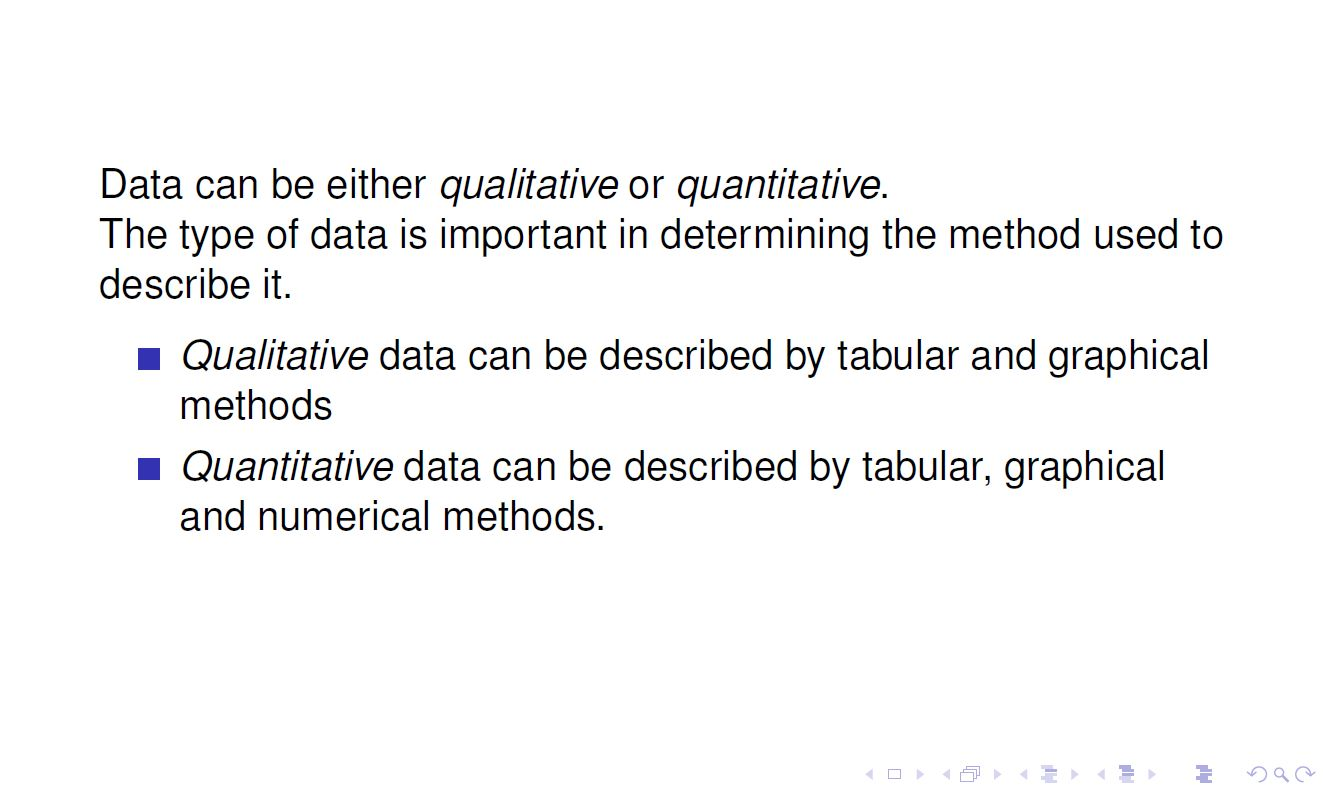
\includegraphics[width=1.1\linewidth]{images/MA4104-Lect03-01}
			\caption{}
			\label{fig:MA4104-Lect03-01}
		\end{figure}
	\end{frame}
	%===========================================================%
	%===========================================================%
	\begin{frame}
		\frametitle{Revision of Science Maths 3}
		\begin{figure}
			\centering
			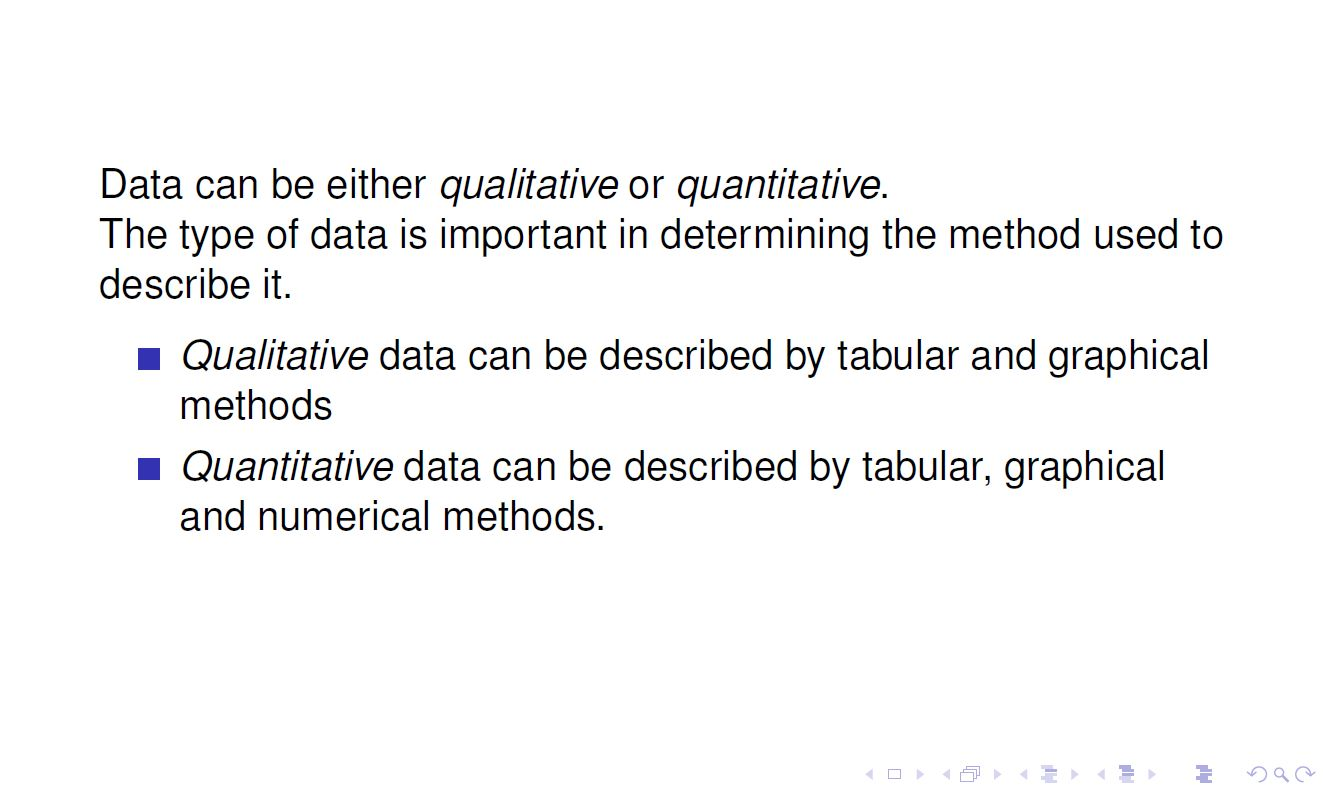
\includegraphics[width=1.1\linewidth]{images/MA4104-Lect03-01}
		\end{figure}
	\end{frame}
	%===========================================================%
	\begin{frame}
		\frametitle{Revision of Science Maths 3}
		\begin{figure}
			\centering
			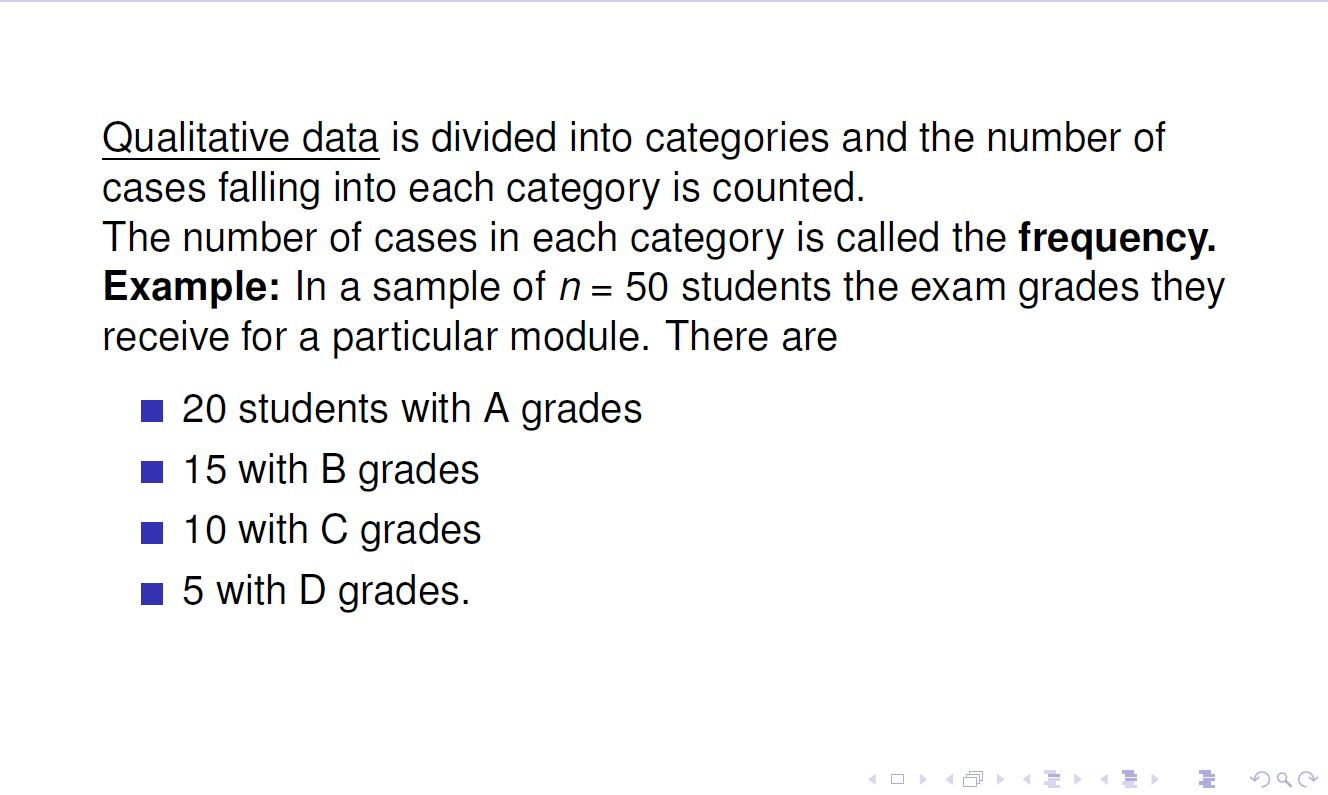
\includegraphics[width=1.1\linewidth]{images/MA4104-Lect03-02}
		\end{figure}
	\end{frame}
	%===========================================================%
	\begin{frame}
		\frametitle{Revision of Science Maths 3}
		\begin{figure}
			\centering
			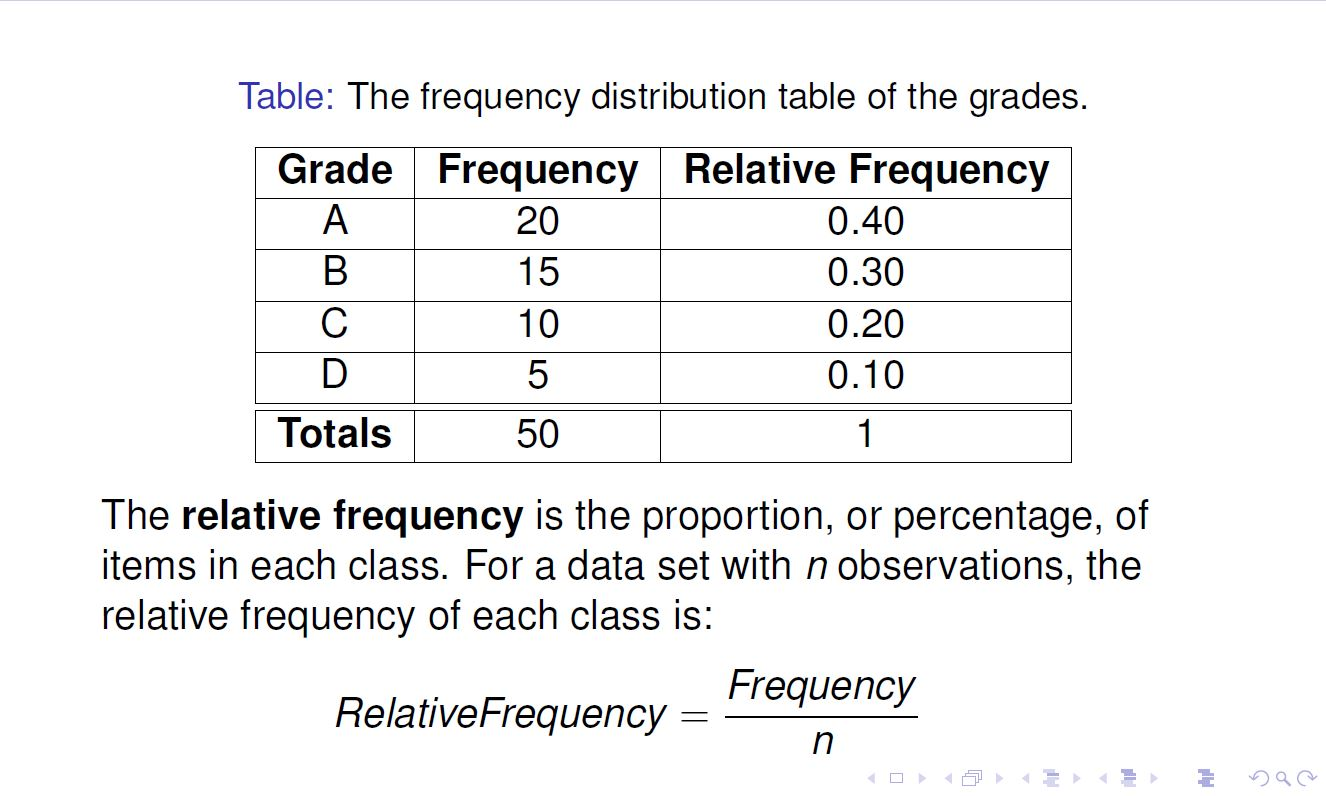
\includegraphics[width=1.1\linewidth]{images/MA4104-Lect03-03}
			
		\end{figure}
	\end{frame}
	%===========================================================%
	\begin{frame}
		\frametitle{Revision of Science Maths 3}
		\begin{figure}
			\centering
			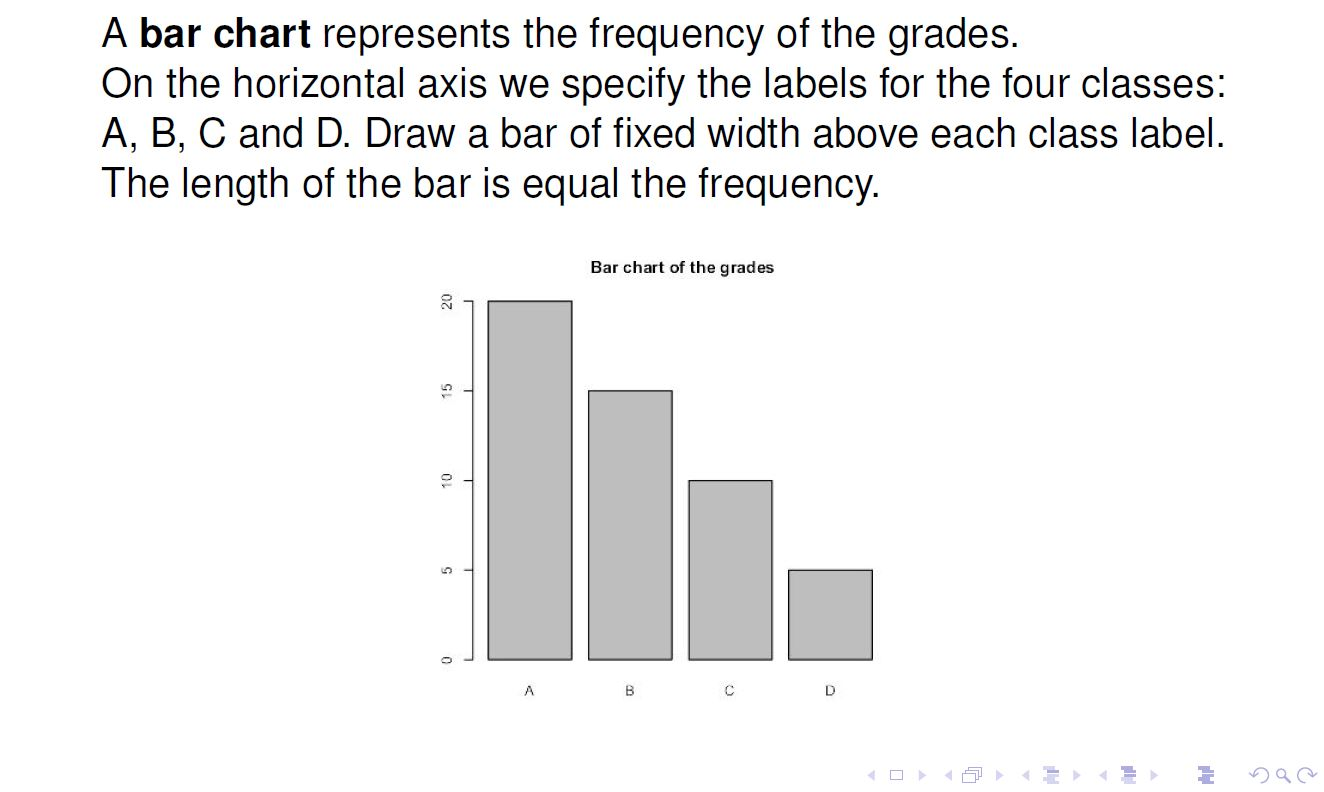
\includegraphics[width=1.1\linewidth]{images/MA4104-Lect03-04}
			
		\end{figure}
	\end{frame}
	%===========================================================%
	\begin{frame}
		\frametitle{Revision of Science Maths 3}
		\begin{figure}
			\centering	
			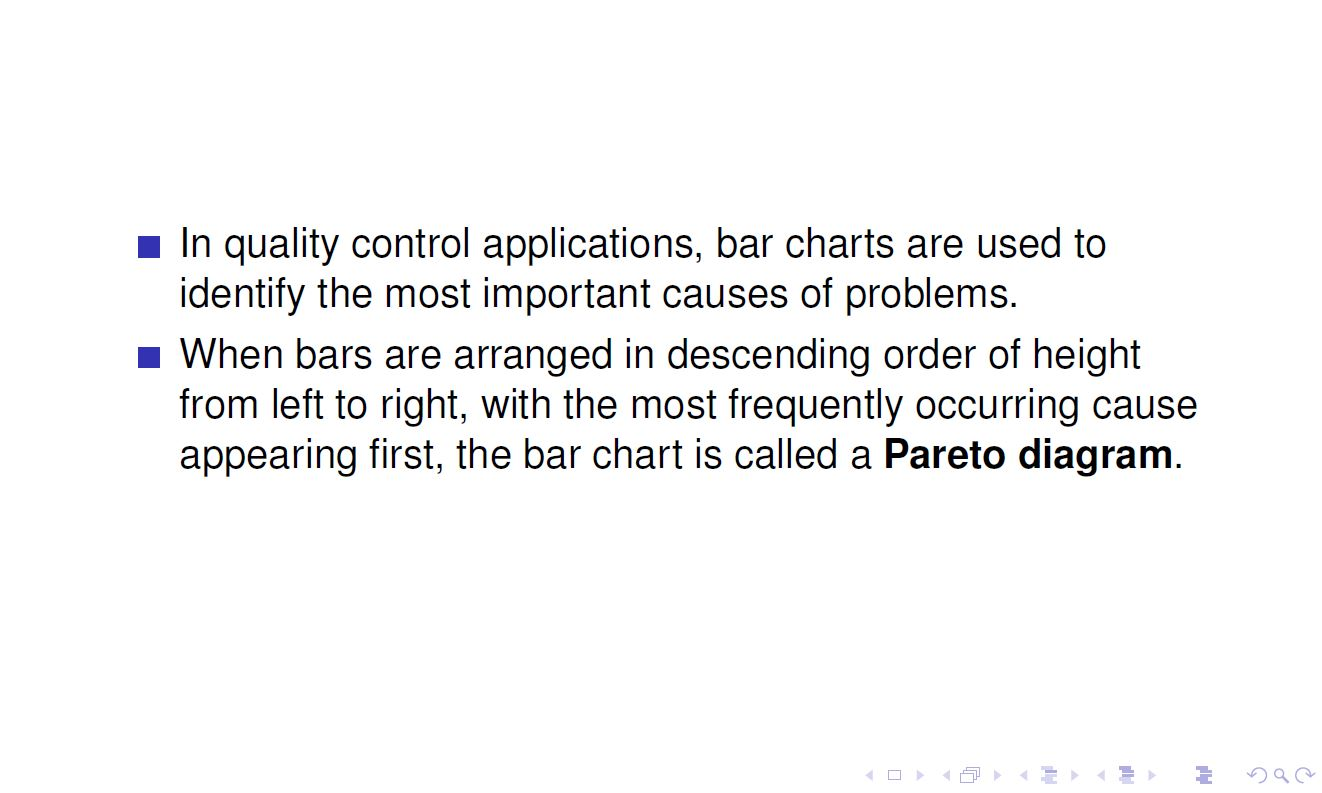
\includegraphics[width=1.1\linewidth]{images/MA4104-Lect03-05}
			
		\end{figure}
	\end{frame}
	%===========================================================%
	\begin{frame}
		\frametitle{Revision of Science Maths 3}
		\begin{figure}
			\centering
			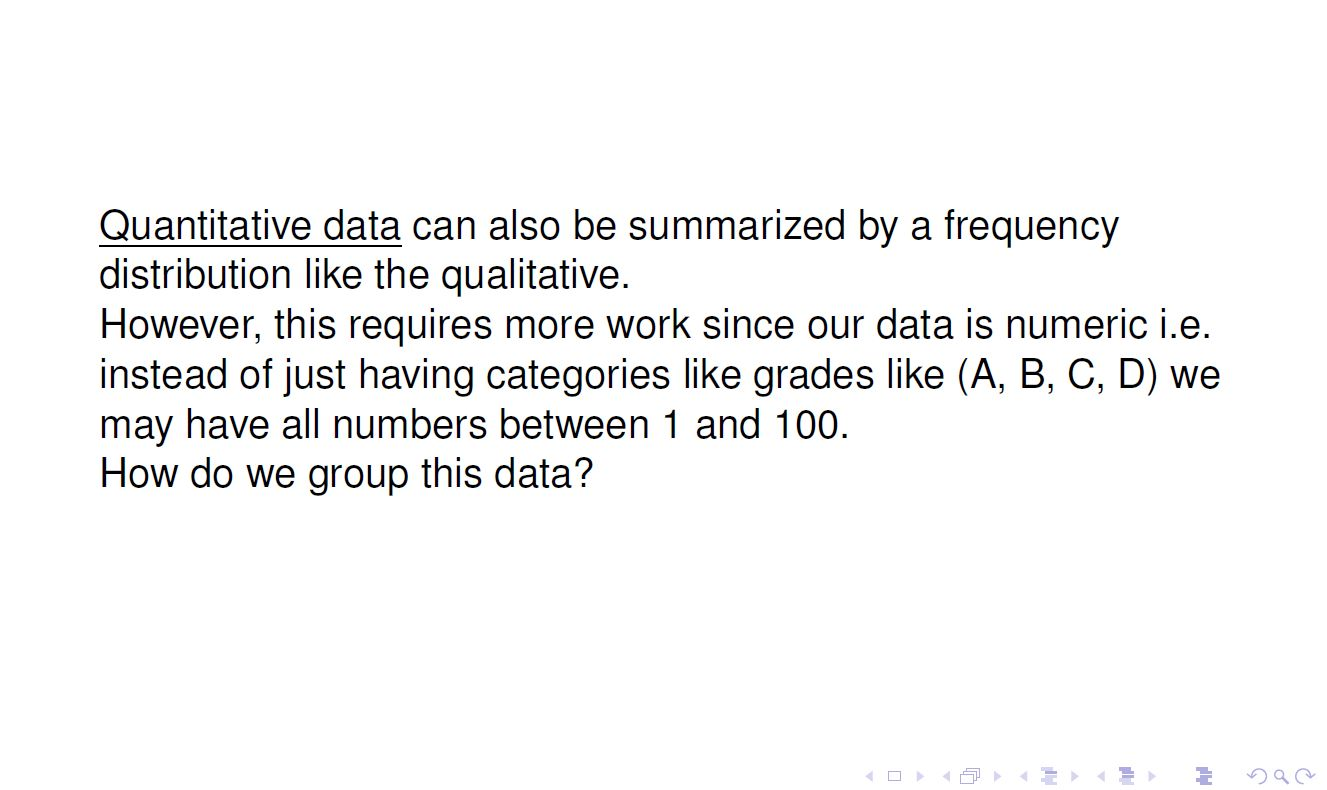
\includegraphics[width=1.1\linewidth]{images/MA4104-Lect03-06}
			
		\end{figure}
	\end{frame}
	%===========================================================%
	\begin{frame}
		\frametitle{Revision of Science Maths 3}
		\begin{figure}
			\centering	
			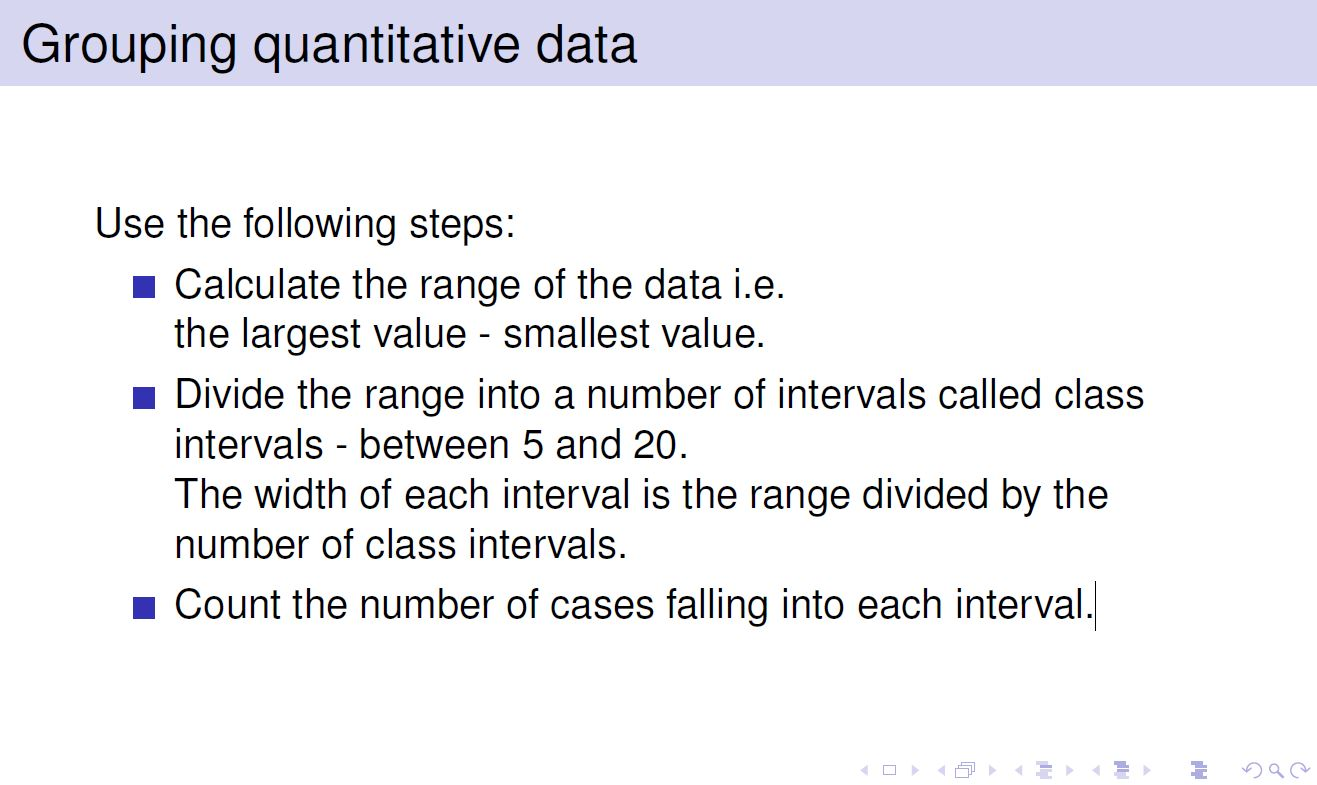
\includegraphics[width=1.1\linewidth]{images/MA4104-Lect03-07}
			
		\end{figure}
	\end{frame}
	%===========================================================%
	\begin{frame}
		\frametitle{Revision of Science Maths 3}
		\begin{figure}
			\centering
			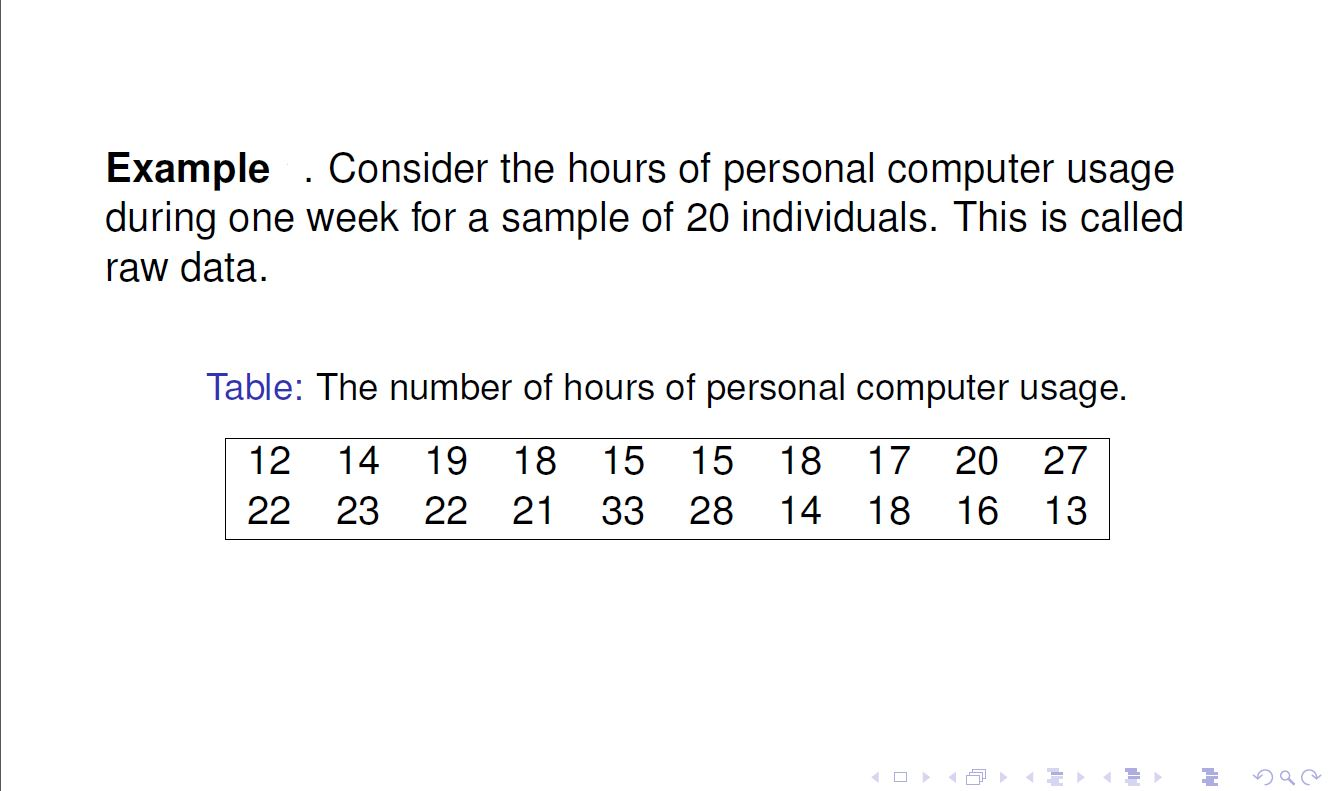
\includegraphics[width=1.1\linewidth]{images/MA4104-Lect03-08}
			
		\end{figure}
	\end{frame}
	%===========================================================%
	\begin{frame}
		\frametitle{Revision of Science Maths 3}
		\begin{figure}
			\centering	
			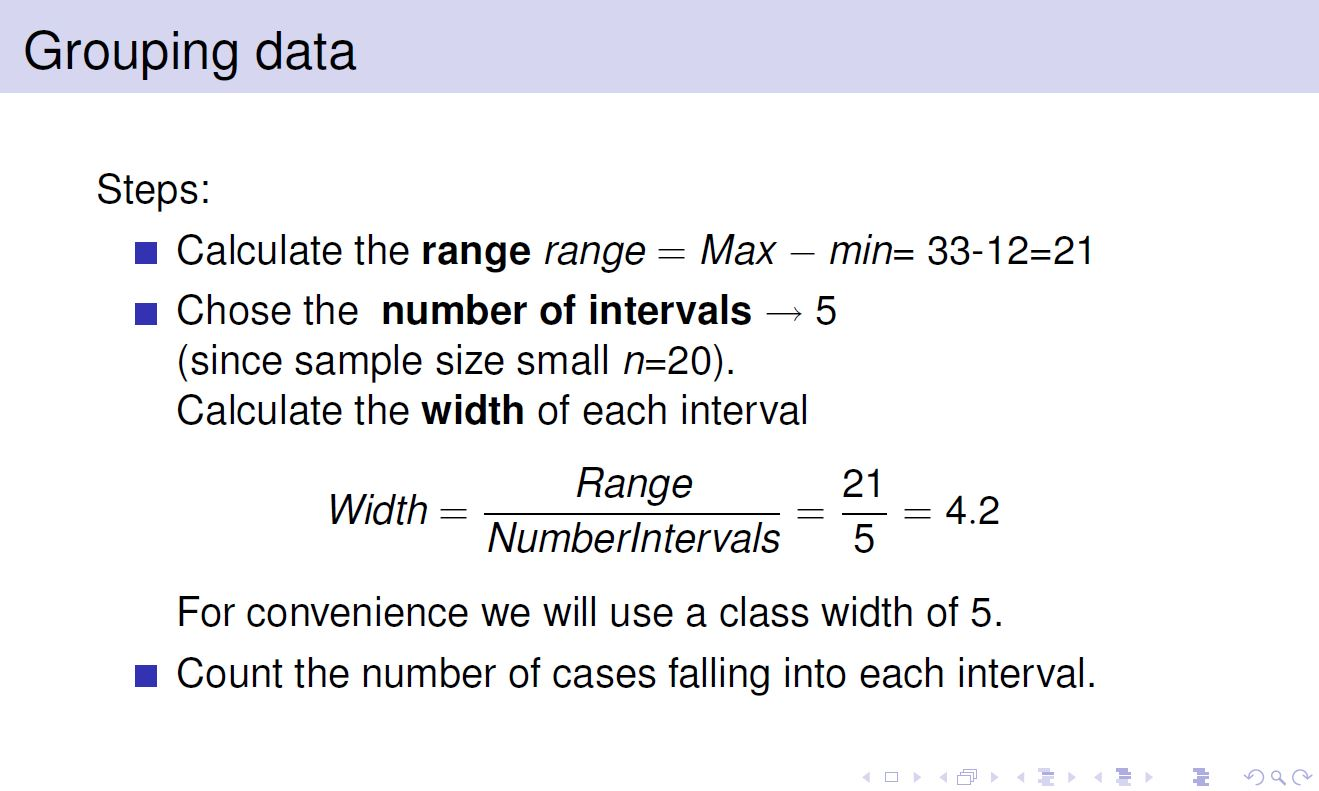
\includegraphics[width=1.1\linewidth]{images/MA4104-Lect03-09}
			
		\end{figure}
	\end{frame}
	%===========================================================%
	\begin{frame}
		\frametitle{Revision of Science Maths 3}
		\begin{figure}
			\centering
			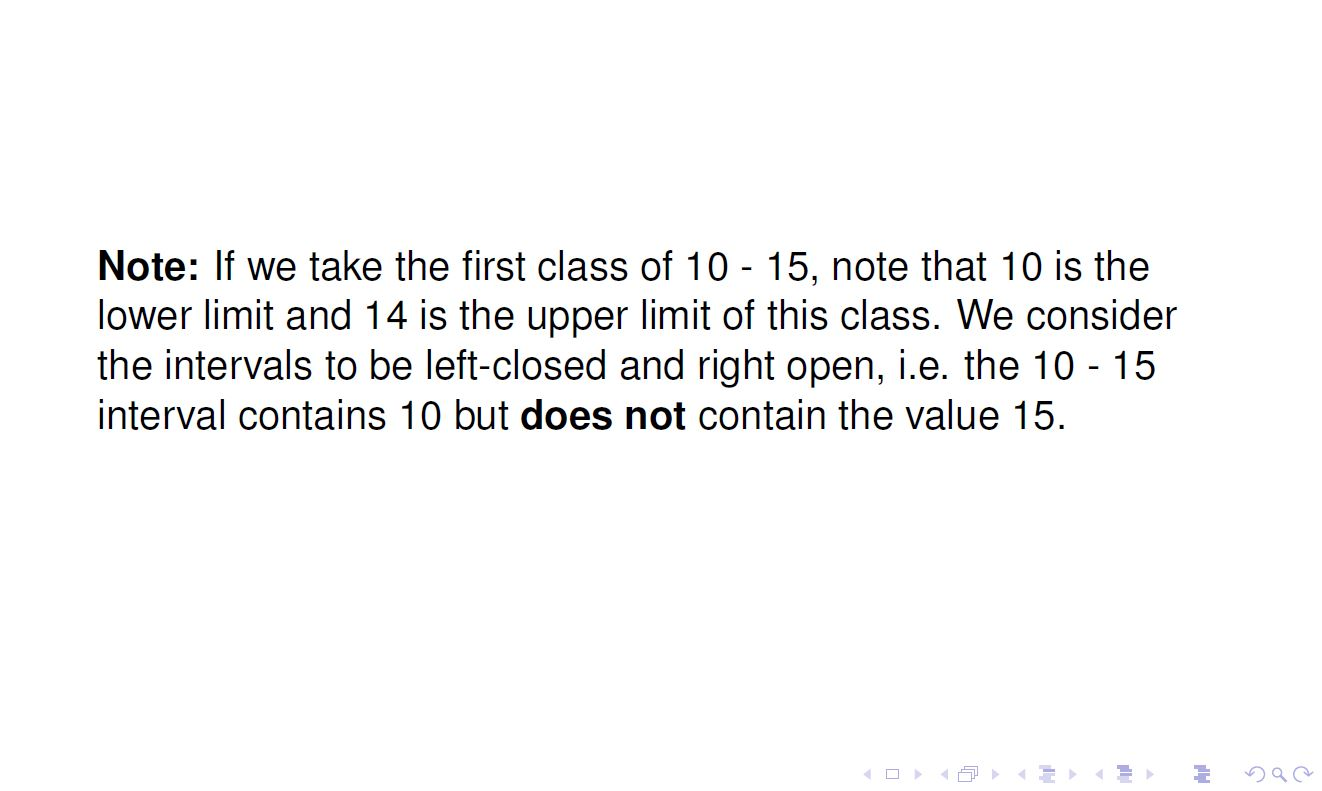
\includegraphics[width=1.1\linewidth]{images/MA4104-Lect03-10}
			
		\end{figure}
	\end{frame}
	%===========================================================%
	\begin{frame}
		\frametitle{Revision of Science Maths 3}
		\begin{figure}
			\centering
			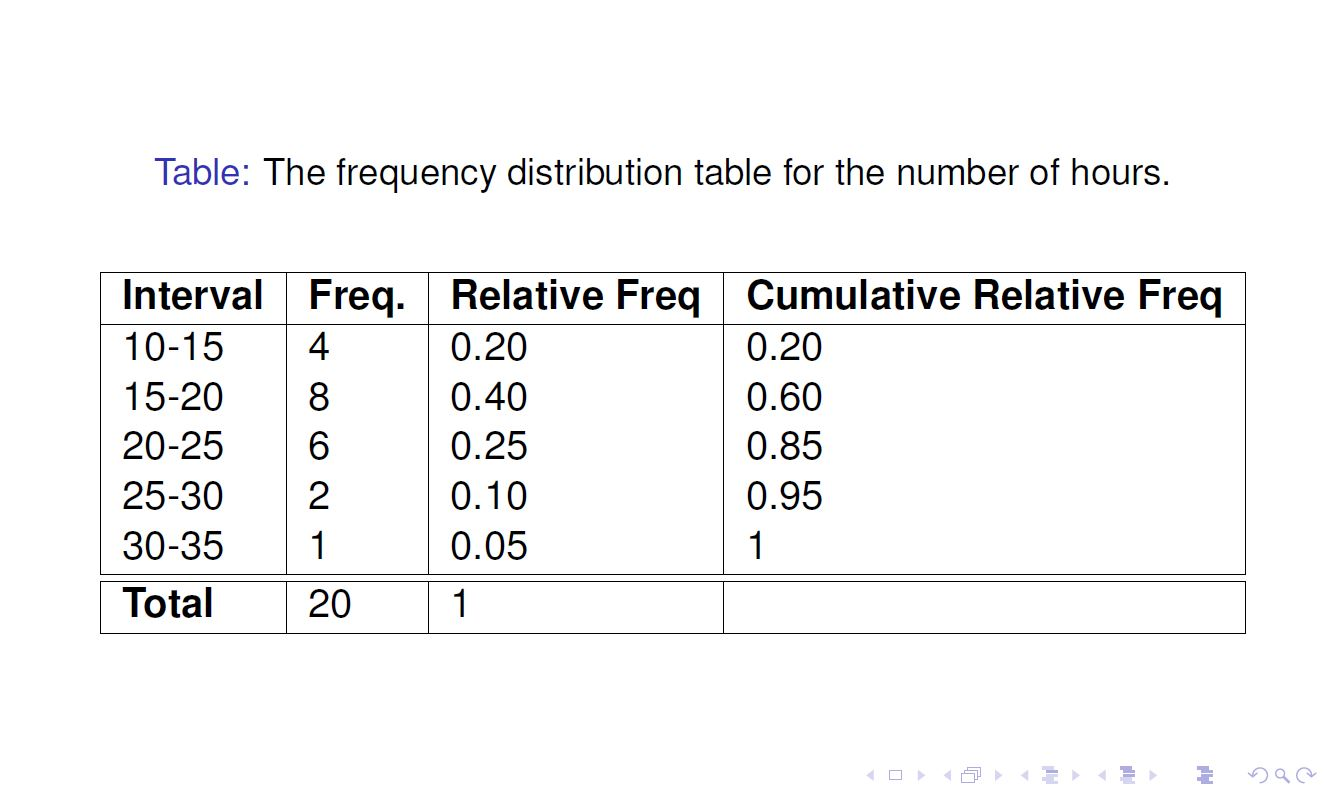
\includegraphics[width=1.1\linewidth]{images/MA4104-Lect03-11}
			
		\end{figure}
	\end{frame}
	%===========================================================%
	\begin{frame}
		\frametitle{Revision of Science Maths 3}
		\begin{figure}
			\centering
			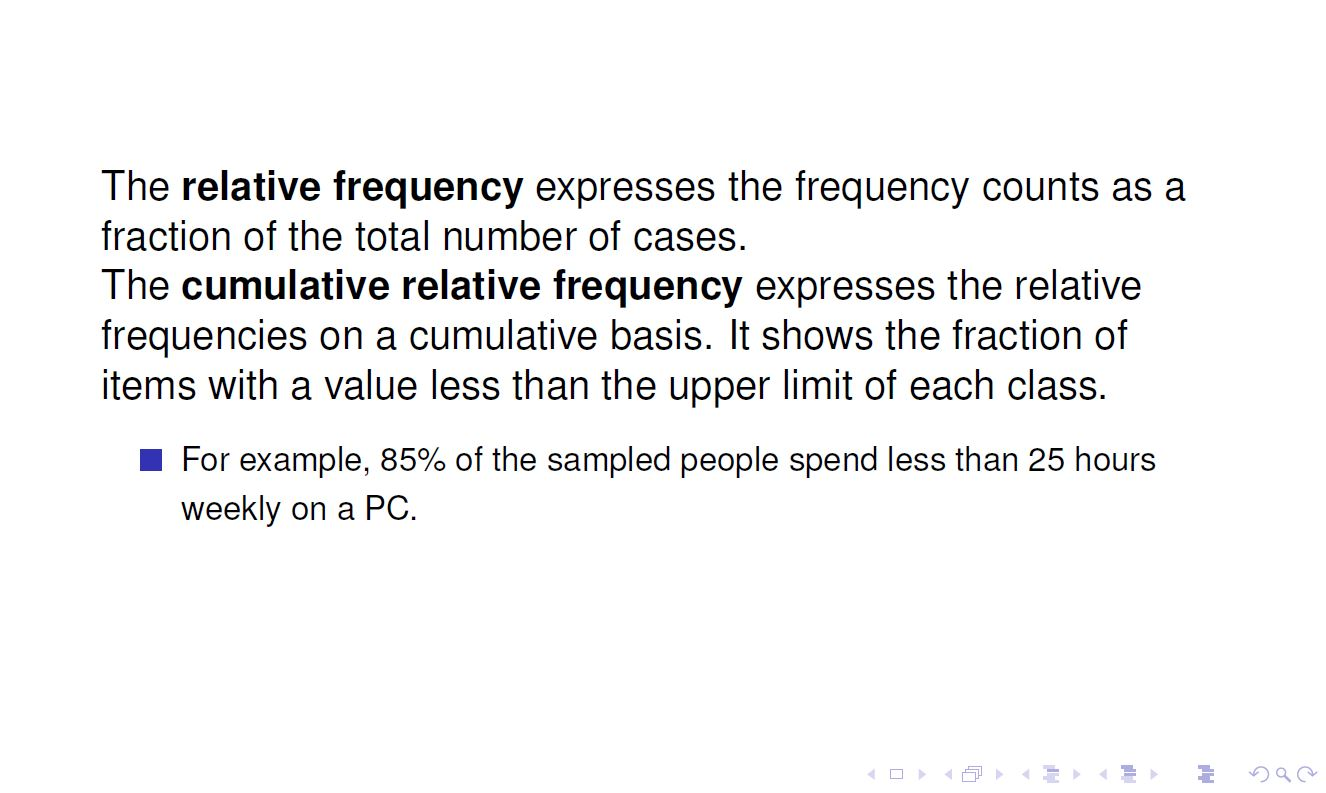
\includegraphics[width=1.1\linewidth]{images/MA4104-Lect03-12}
			
		\end{figure}
	\end{frame}
	%===========================================================%
	\begin{frame}
		\frametitle{Revision of Science Maths 3}
		\begin{figure}
			\centering
			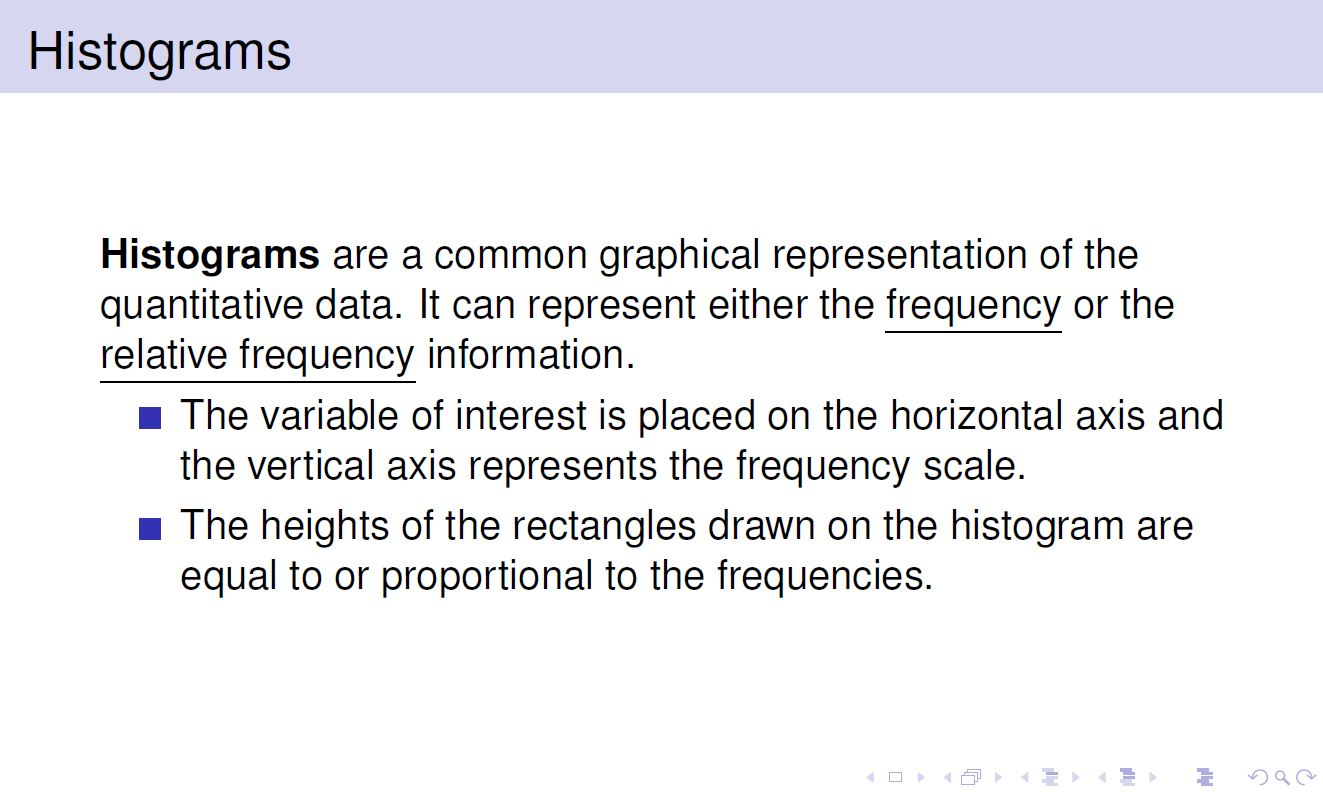
\includegraphics[width=1.1\linewidth]{images/MA4104-Lect03-13}
			
		\end{figure}
	\end{frame}
	%===========================================================%
	\begin{frame}
		\frametitle{Revision of Science Maths 3}
		\begin{figure}
			\centering	
			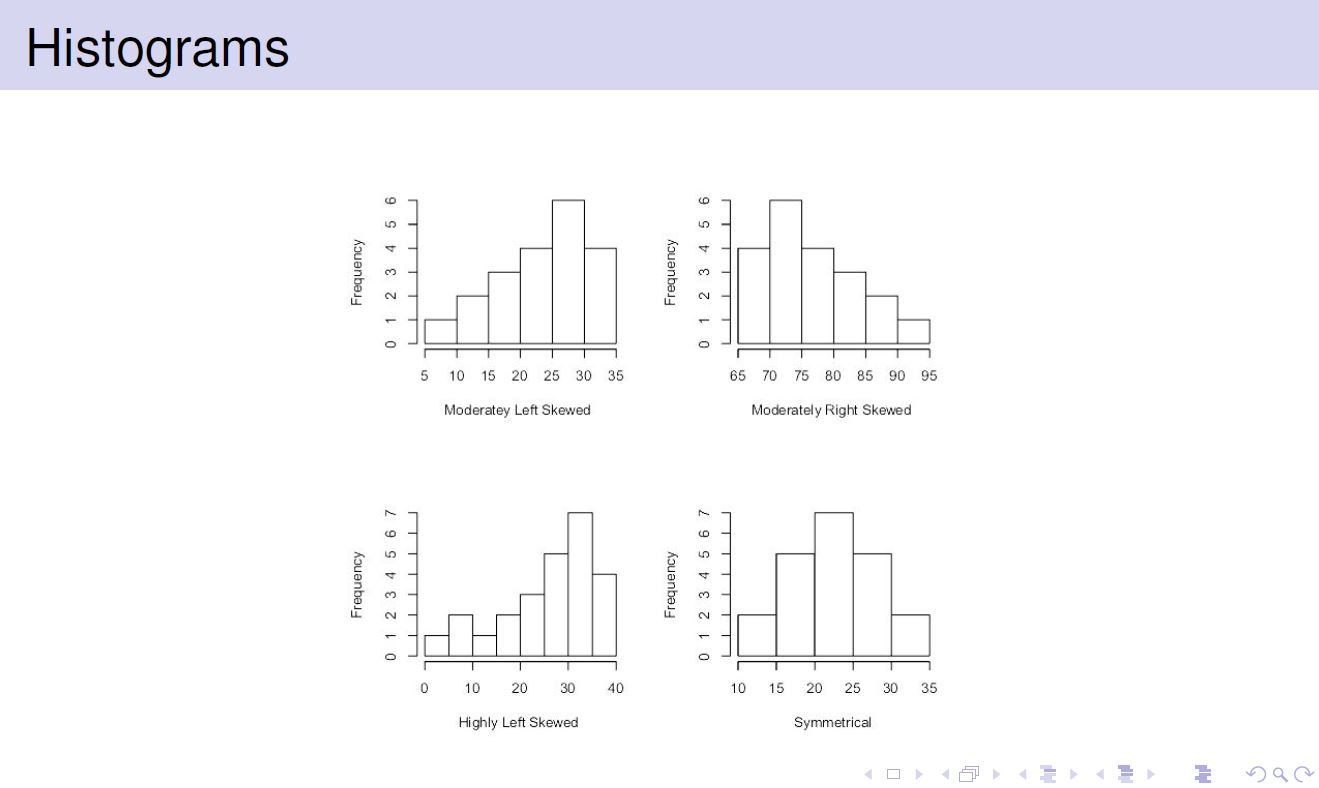
\includegraphics[width=1.1\linewidth]{images/MA4104-Lect03-14}
			
		\end{figure}
	\end{frame}
	%===========================================================%
	\begin{frame}
		\frametitle{Revision of Science Maths 3}
		\begin{figure}
			\centering
			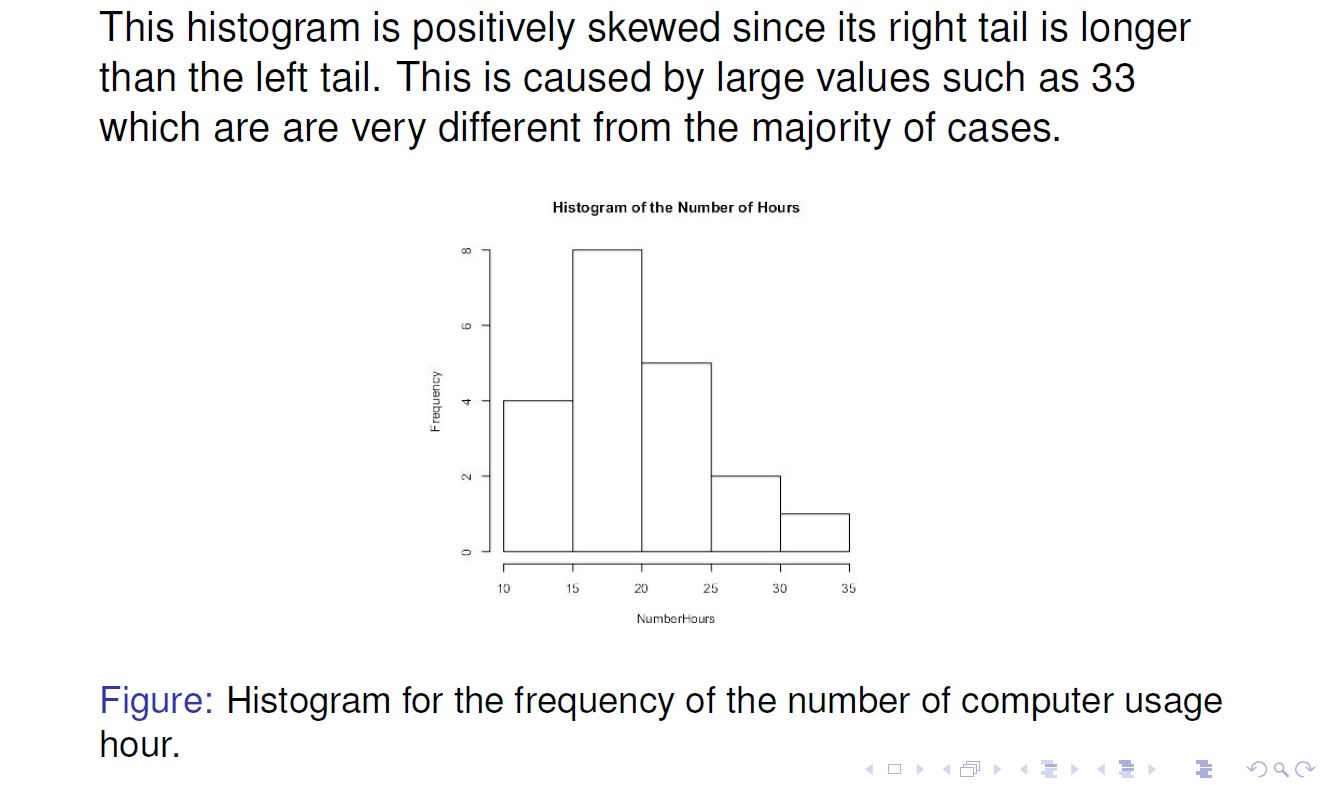
\includegraphics[width=1.1\linewidth]{images/MA4104-Lect03-15}
			
		\end{figure}
	\end{frame}
	%===========================================================%
	\begin{frame}
		\frametitle{Revision of Science Maths 3}
		\begin{figure}
			\centering
			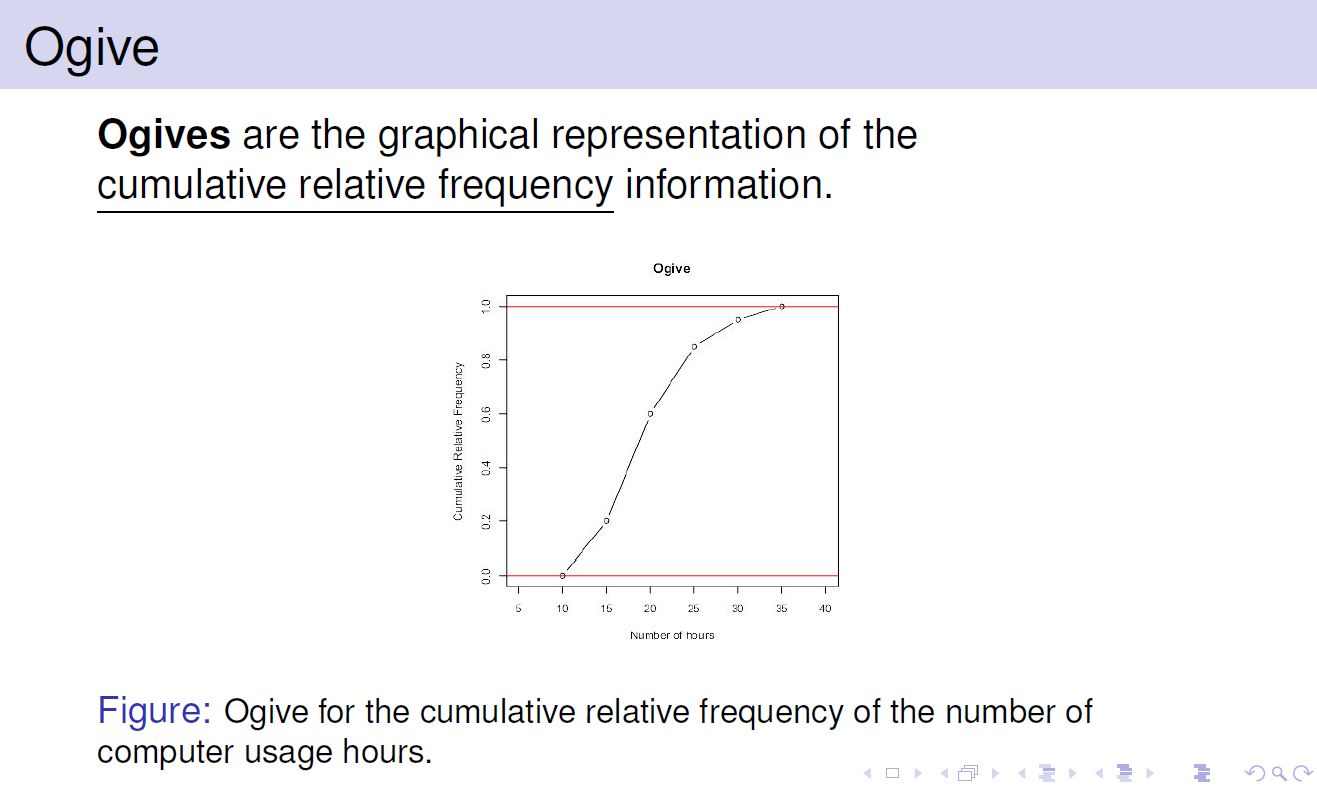
\includegraphics[width=1.1\linewidth]{images/MA4104-Lect03-16}
			
		\end{figure}
	\end{frame}
	%===========================================================%
	\begin{frame}
		\frametitle{Revision of Science Maths 3}
		\begin{figure}
			\centering
			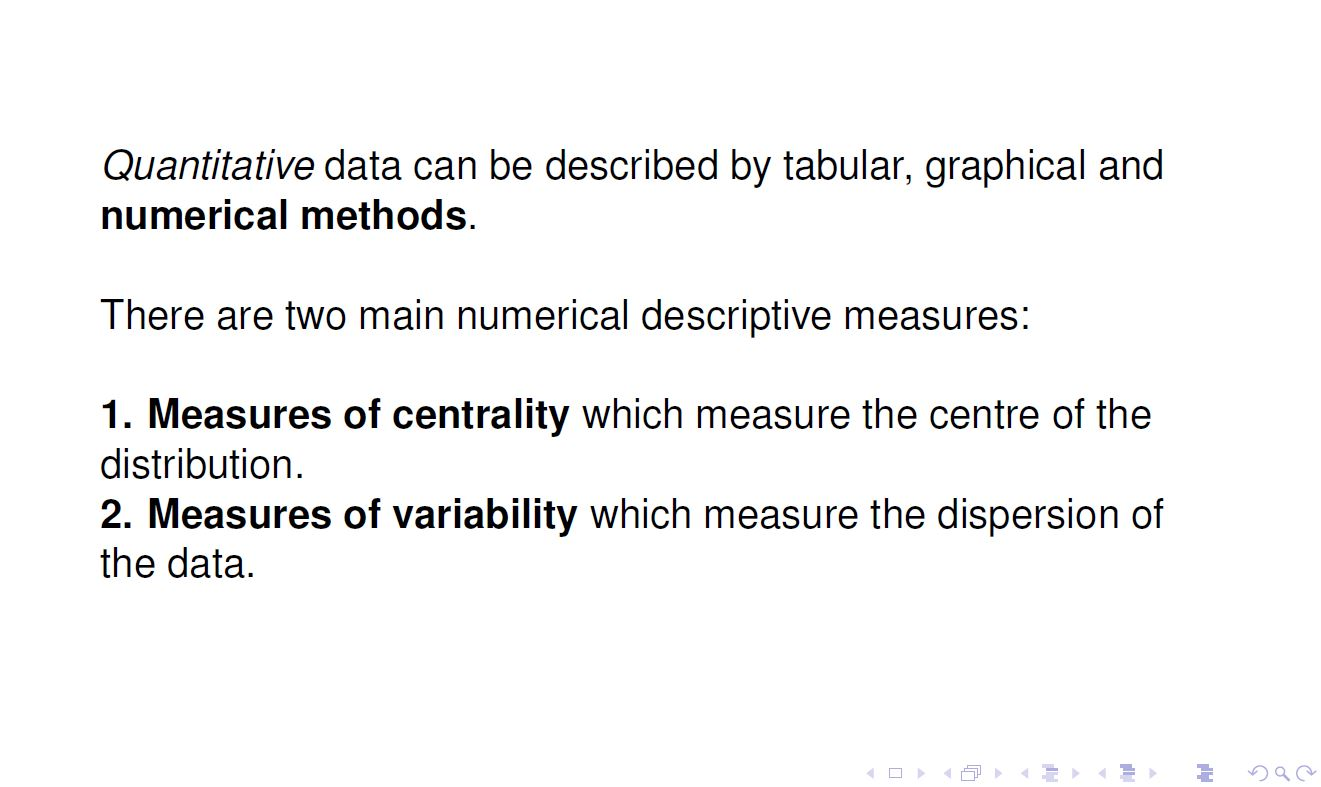
\includegraphics[width=1.1\linewidth]{images/MA4104-Lect04-01}
			
		\end{figure}
	\end{frame}
	%===========================================================%
	\begin{frame}
		\frametitle{Revision of Science Maths 3}
		\begin{figure}
			\centering
			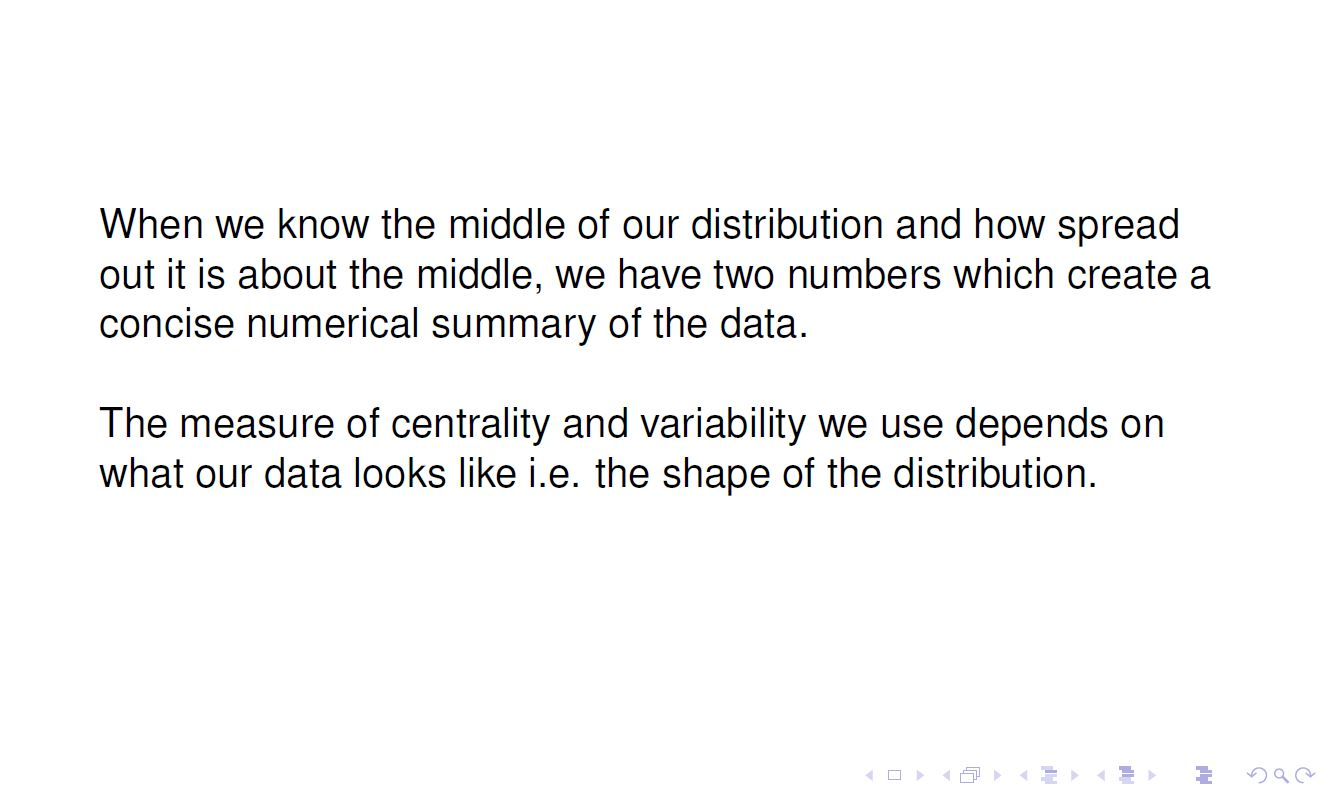
\includegraphics[width=1.1\linewidth]{images/MA4104-Lect04-02}
			
		\end{figure}
	\end{frame}
	%===========================================================%
	\begin{frame}
		\frametitle{Revision of Science Maths 3}
		\begin{figure}
			\centering
			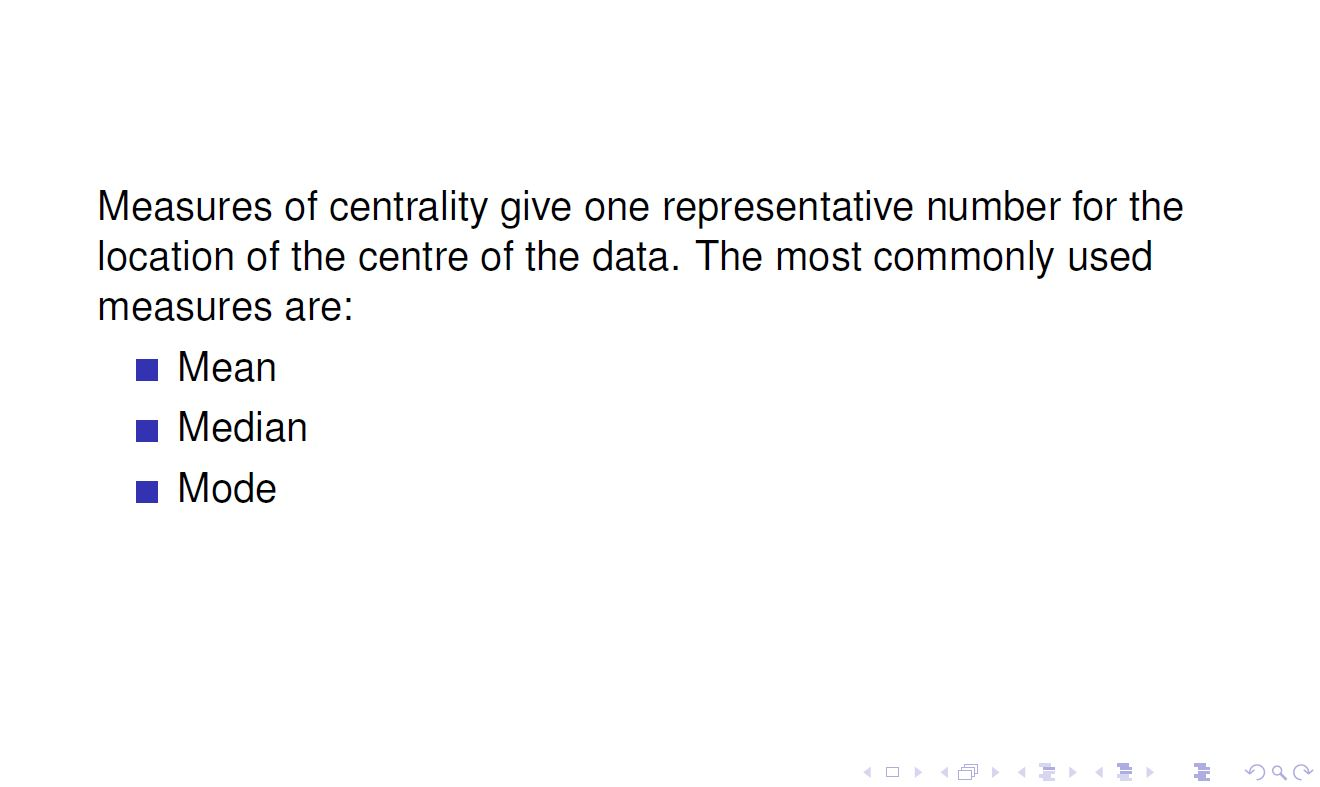
\includegraphics[width=1.1\linewidth]{images/MA4104-Lect04-03}
			
		\end{figure}
	\end{frame}
	%===========================================================%
	\begin{frame}
		\frametitle{Revision of Science Maths 3}
		\begin{figure}
			\centering
			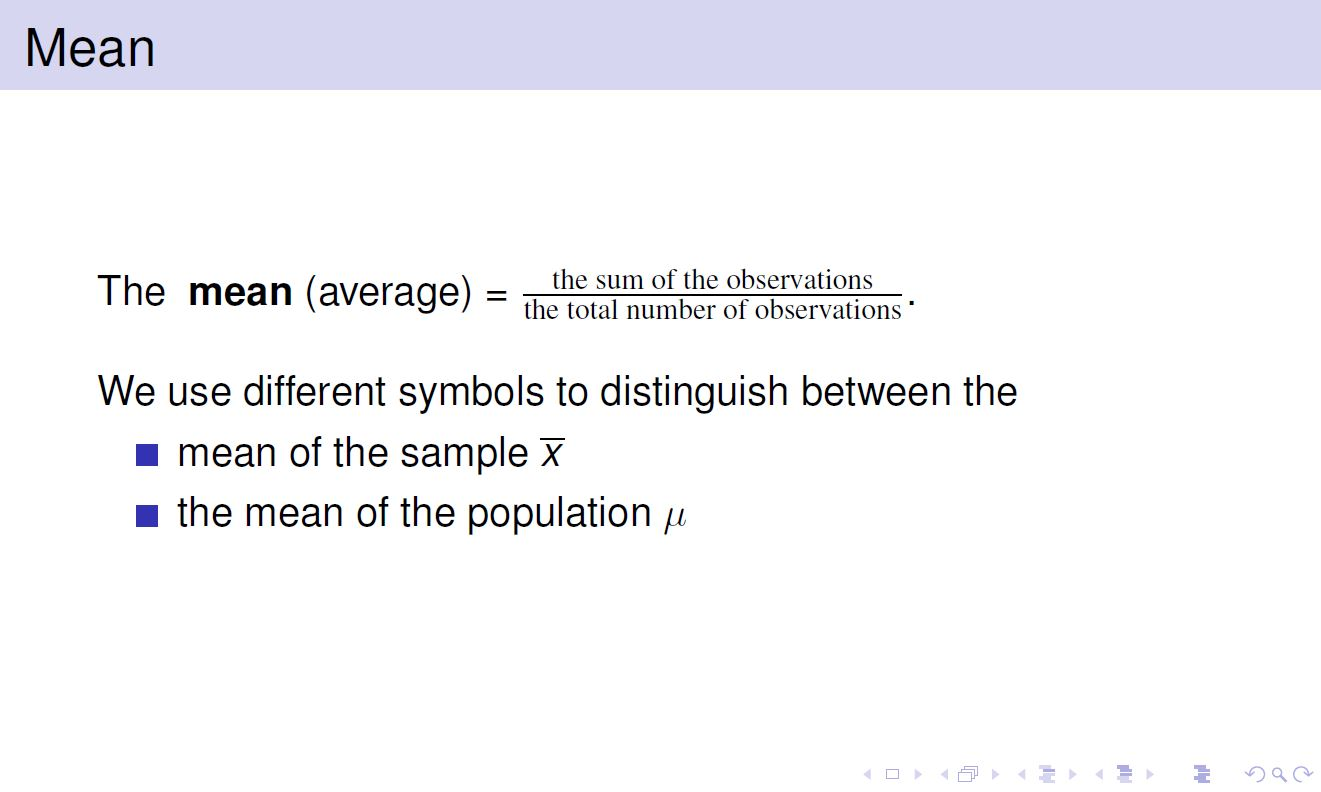
\includegraphics[width=1.1\linewidth]{images/MA4104-Lect04-04}
			
		\end{figure}
	\end{frame}
	%===========================================================%
	\begin{frame}
		\frametitle{Revision of Science Maths 3}
		\begin{figure}
			\centering
			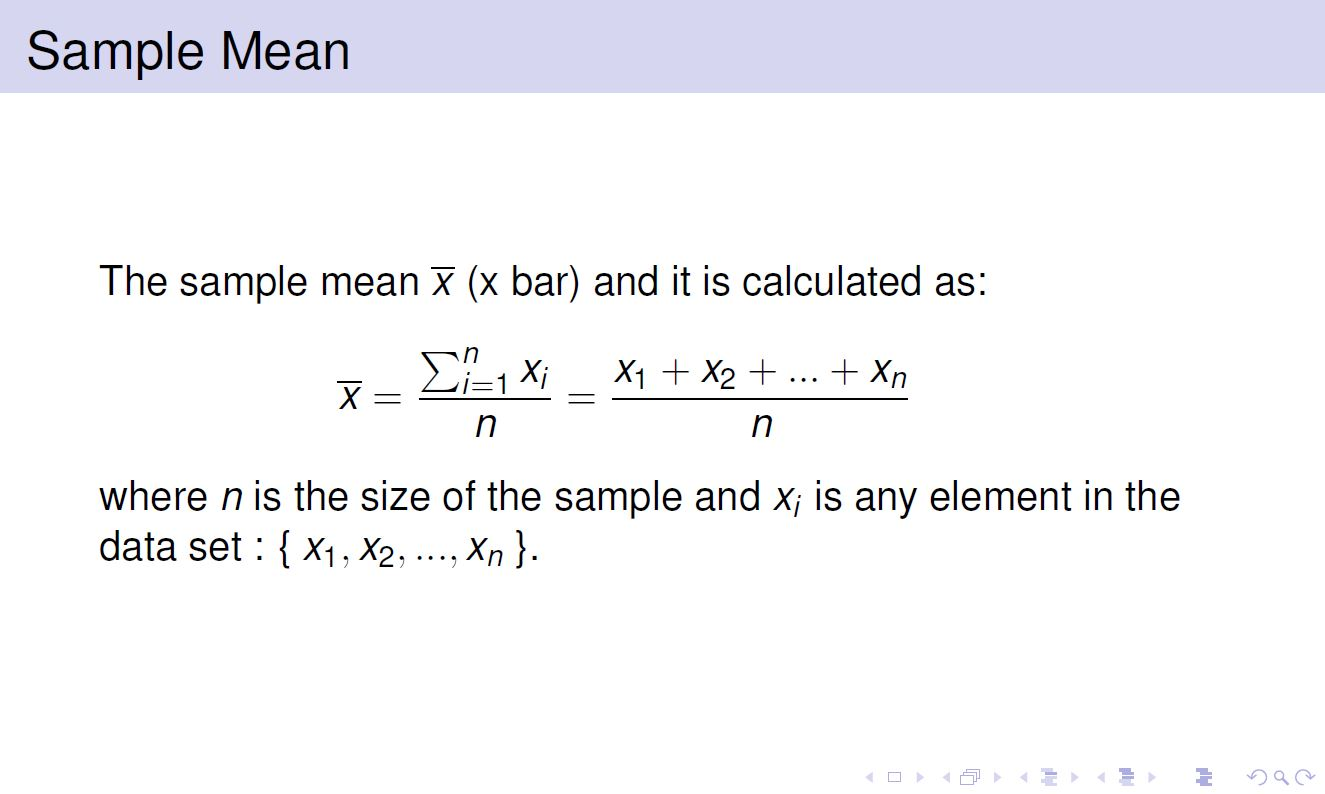
\includegraphics[width=1.1\linewidth]{images/MA4104-Lect04-05}
			
		\end{figure}
	\end{frame}
	%===========================================================%
	\begin{frame}
		\frametitle{Revision of Science Maths 3}
		\begin{figure}
			\centering
			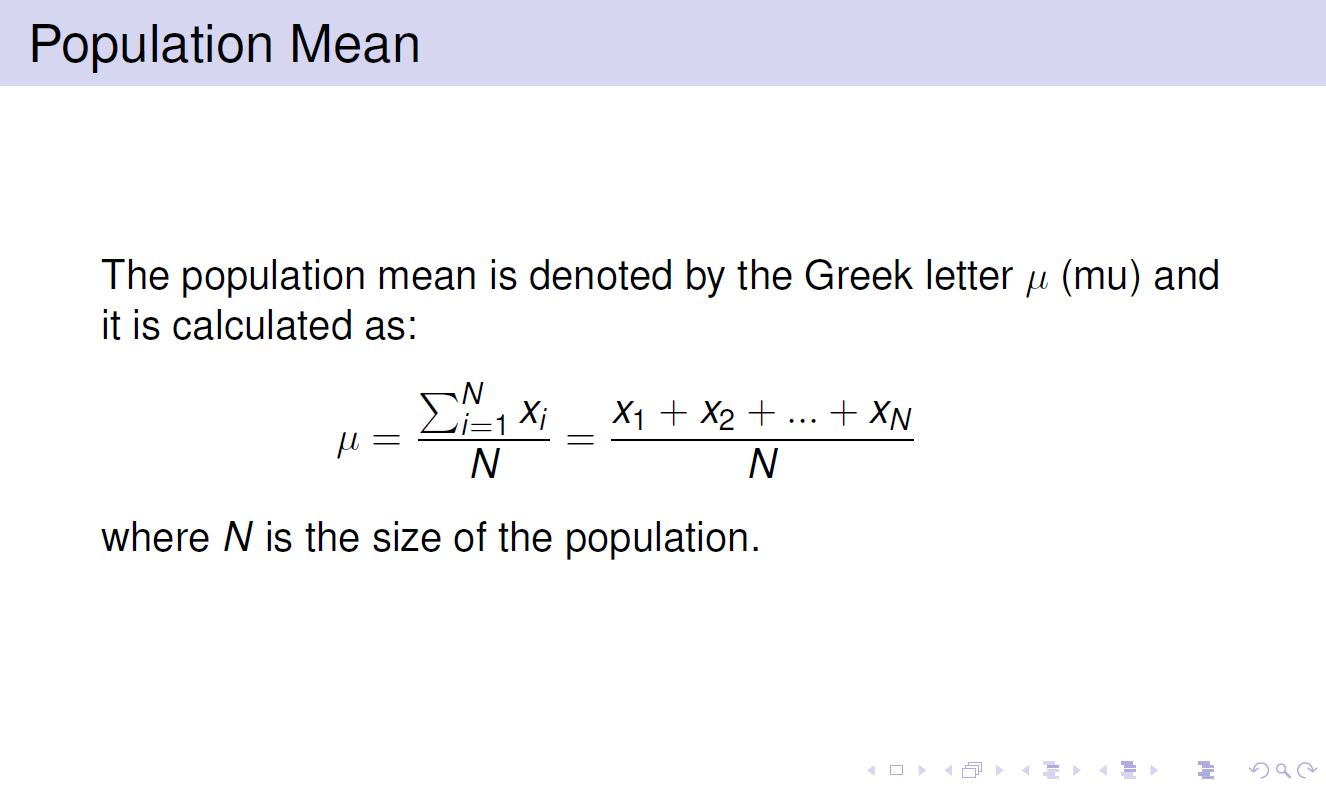
\includegraphics[width=1.1\linewidth]{images/MA4104-Lect04-06}
			
		\end{figure}
	\end{frame}
	%===========================================================%
	\begin{frame}
		\frametitle{Revision of Science Maths 3}
		\begin{figure}
			\centering
			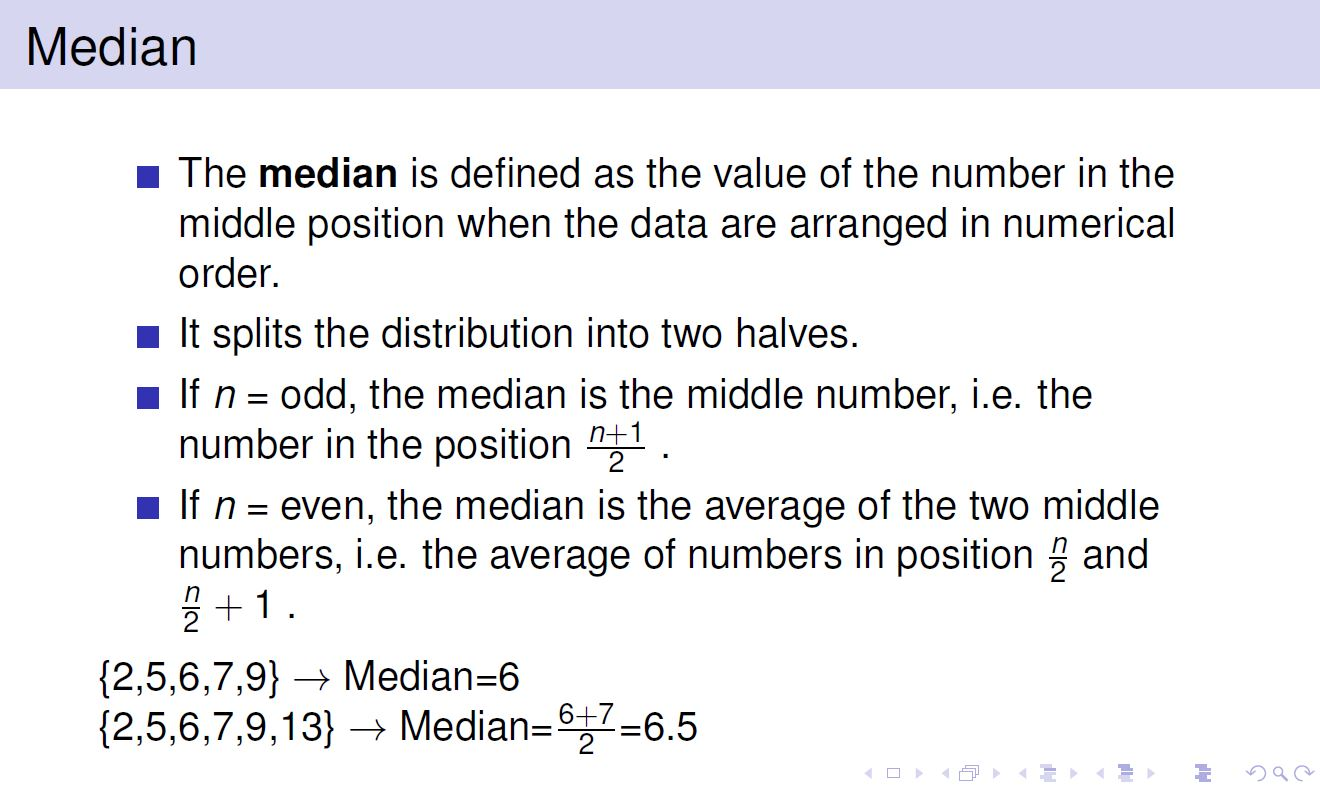
\includegraphics[width=1.1\linewidth]{images/MA4104-Lect04-07}
			
		\end{figure}
	\end{frame}
	%===========================================================%
	\begin{frame}
		\frametitle{Revision of Science Maths 3}
		\begin{figure}
			\centering	
			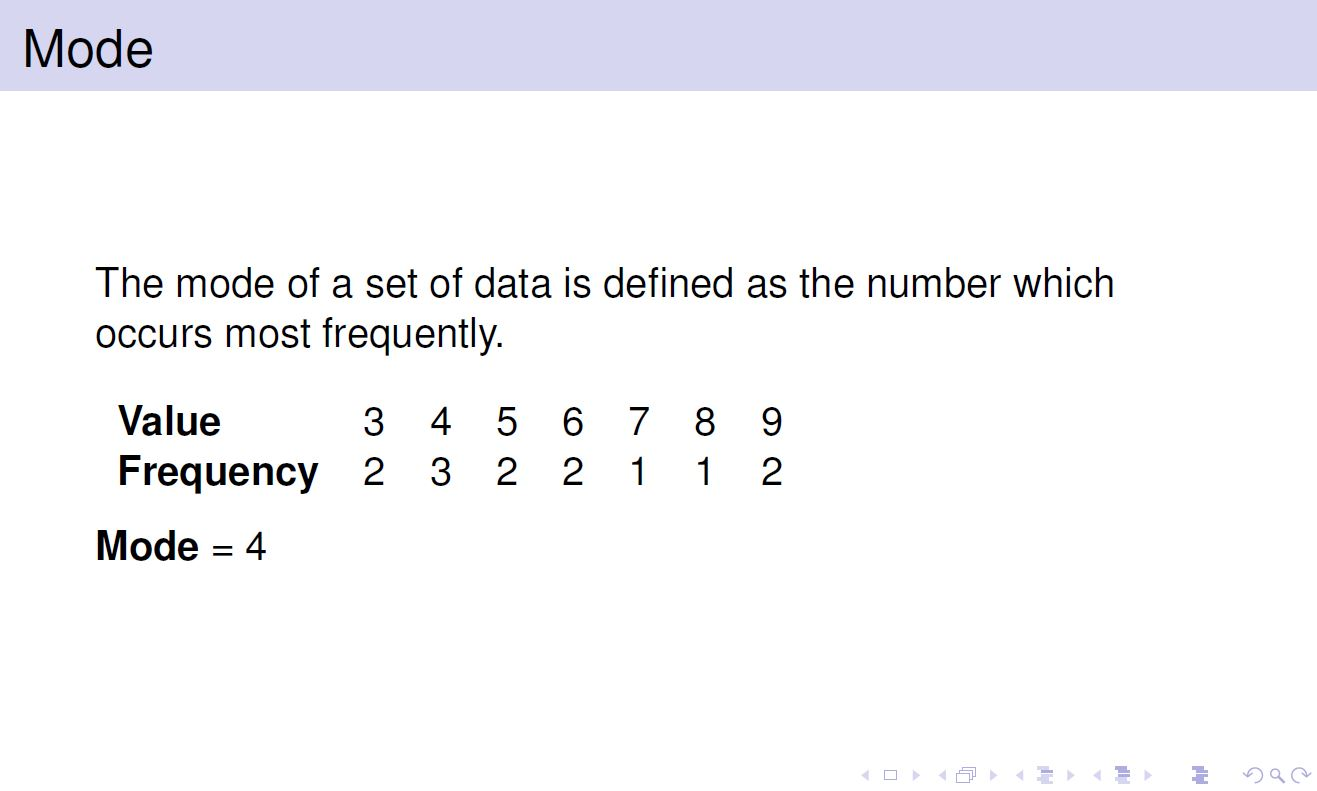
\includegraphics[width=1.1\linewidth]{images/MA4104-Lect04-08}
			
		\end{figure}
	\end{frame}
	%===========================================================%
	\begin{frame}
		\frametitle{Revision of Science Maths 3}
		\begin{figure}
			\centering
			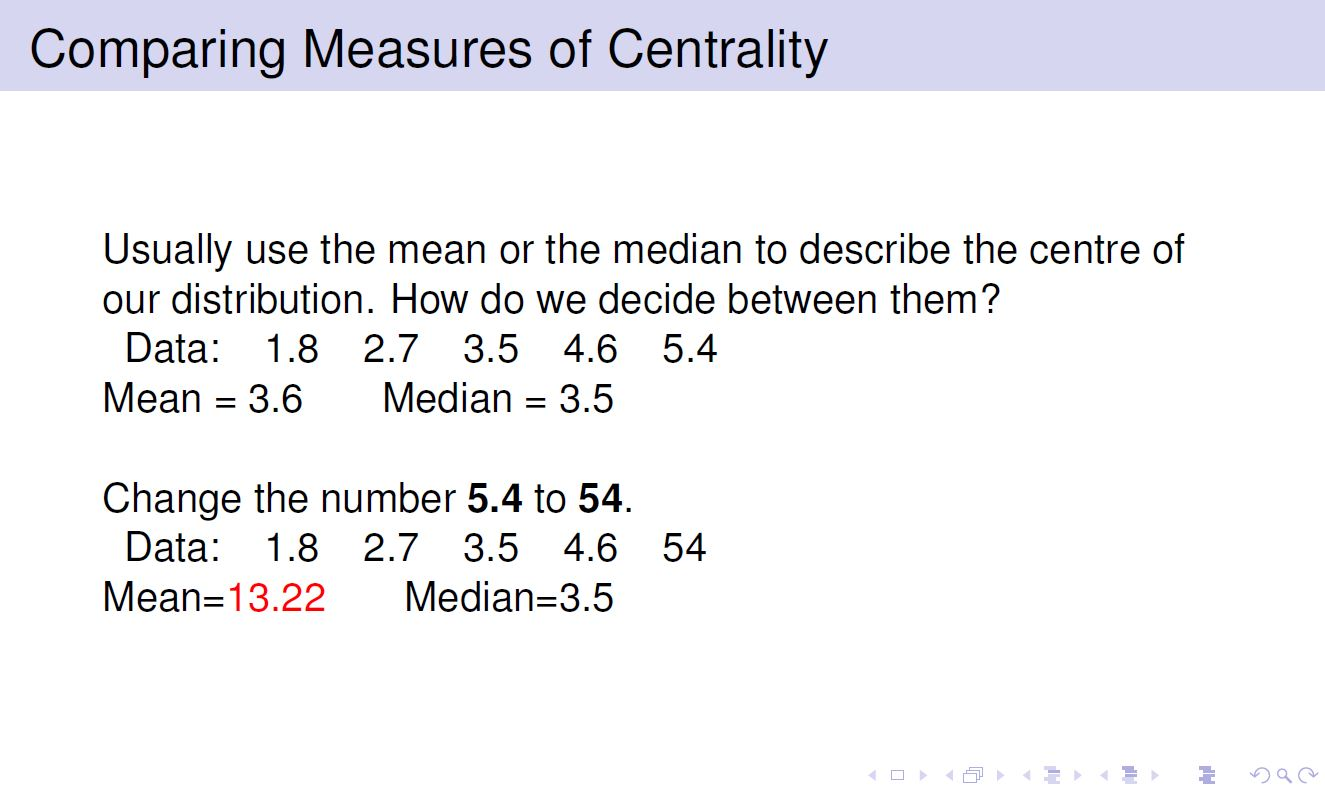
\includegraphics[width=1.1\linewidth]{images/MA4104-Lect04-09}
			
		\end{figure}
	\end{frame}
	%===========================================================%
	\begin{frame}
		\frametitle{Revision of Science Maths 3}
		\begin{figure}
			\centering
			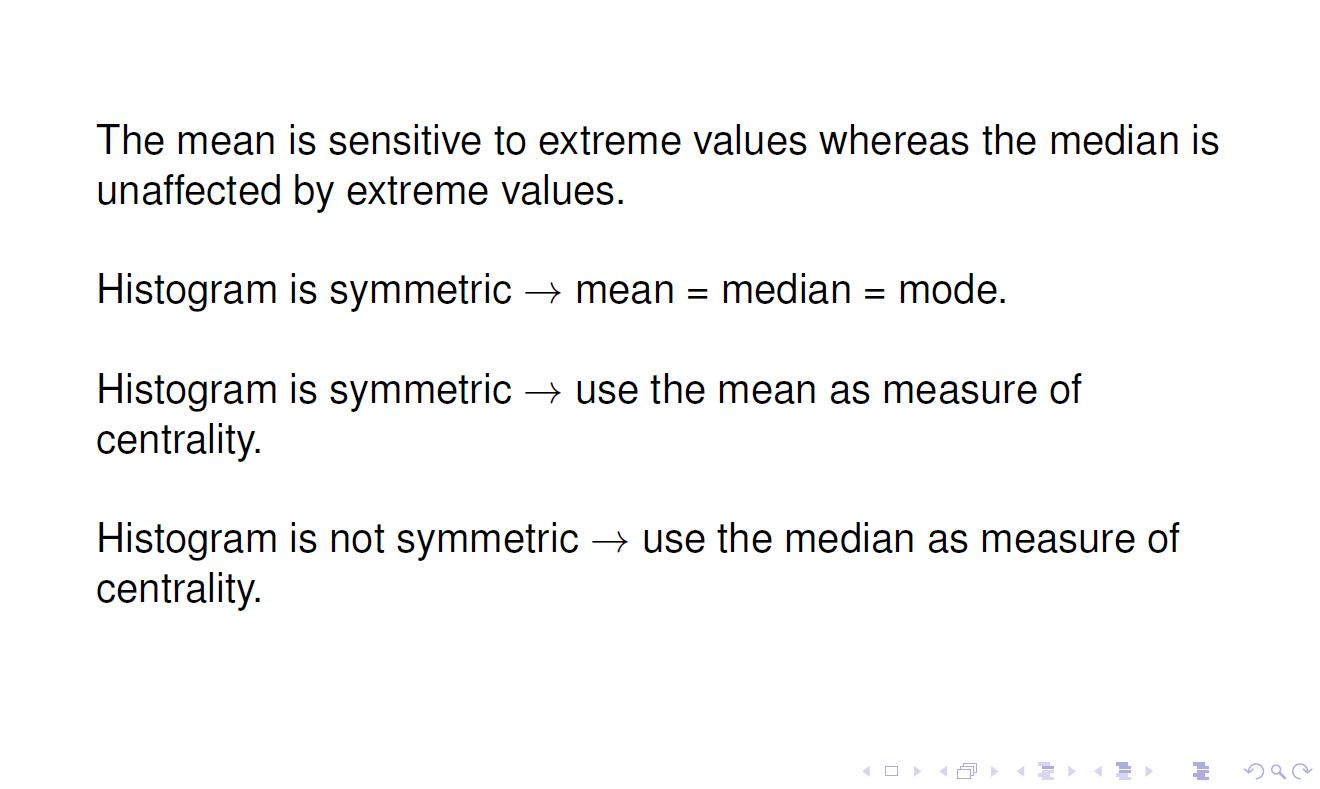
\includegraphics[width=1.1\linewidth]{images/MA4104-Lect04-10}
			
		\end{figure}
	\end{frame}
	%===========================================================%
	\begin{frame}
		\frametitle{Revision of Science Maths 3}
		\begin{figure}
			\centering
			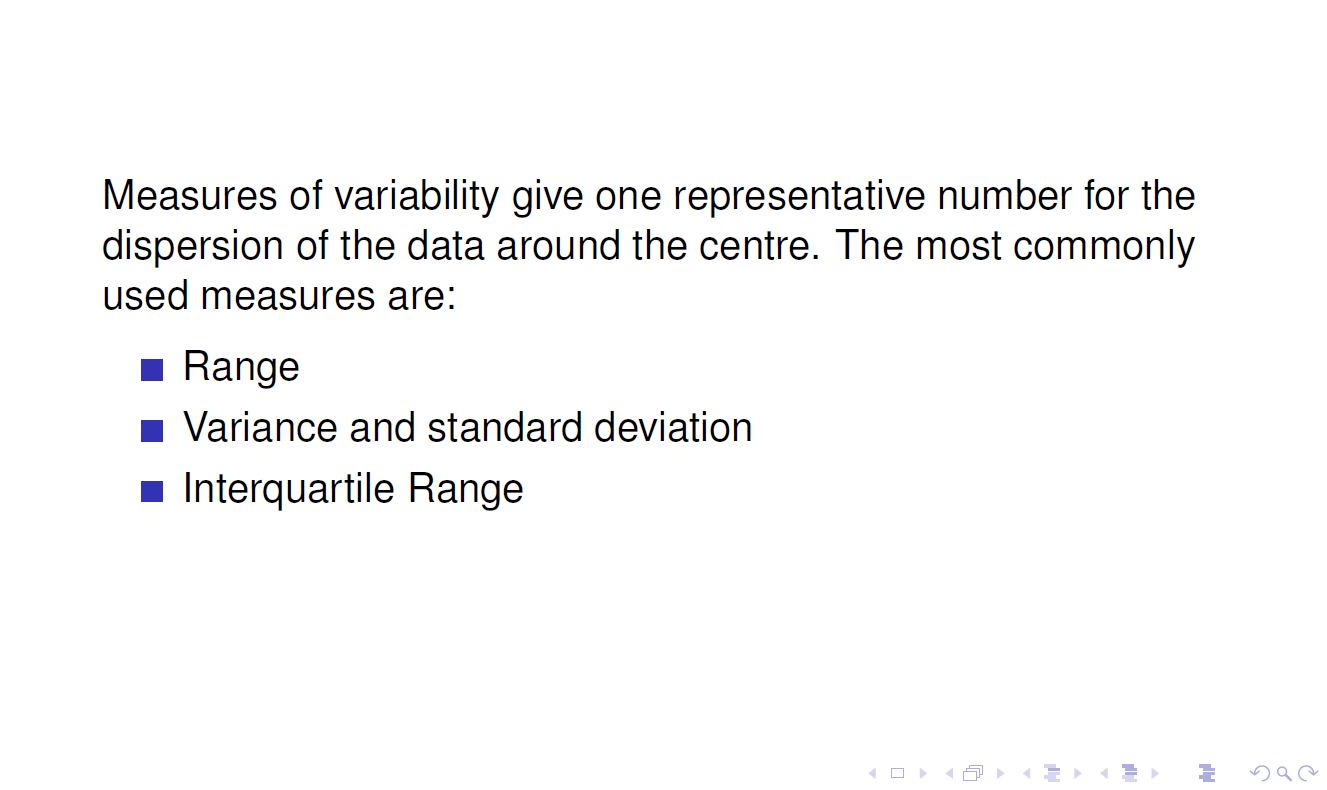
\includegraphics[width=1.1\linewidth]{images/MA4104-Lect04-11}
			
		\end{figure}
	\end{frame}
	%===========================================================%
	\begin{frame}
		\frametitle{Revision of Science Maths 3}
		\begin{figure}
			\centering
			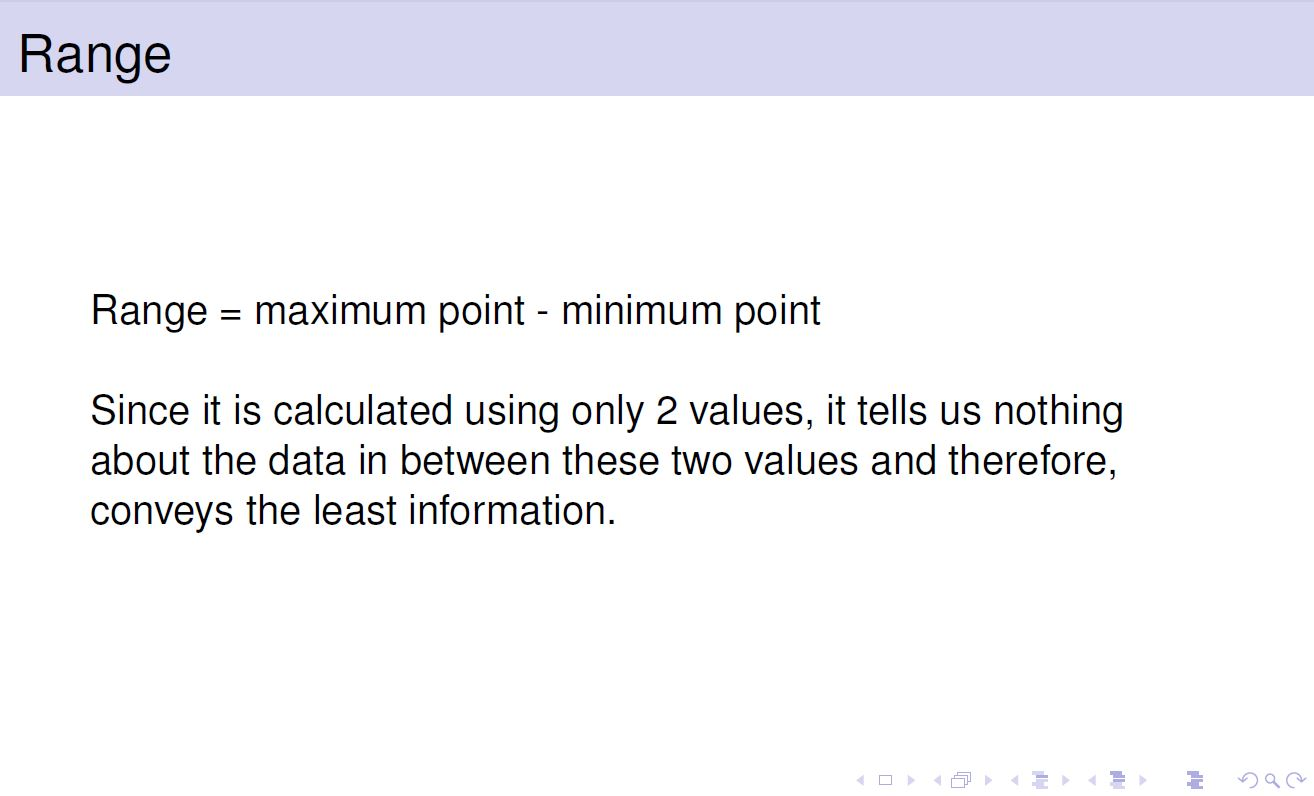
\includegraphics[width=1.1\linewidth]{images/MA4104-Lect04-12}
			
		\end{figure}
	\end{frame}
	%===========================================================%
	\begin{frame}
		\frametitle{Revision of Science Maths 3}
		\begin{figure}
			\centering
			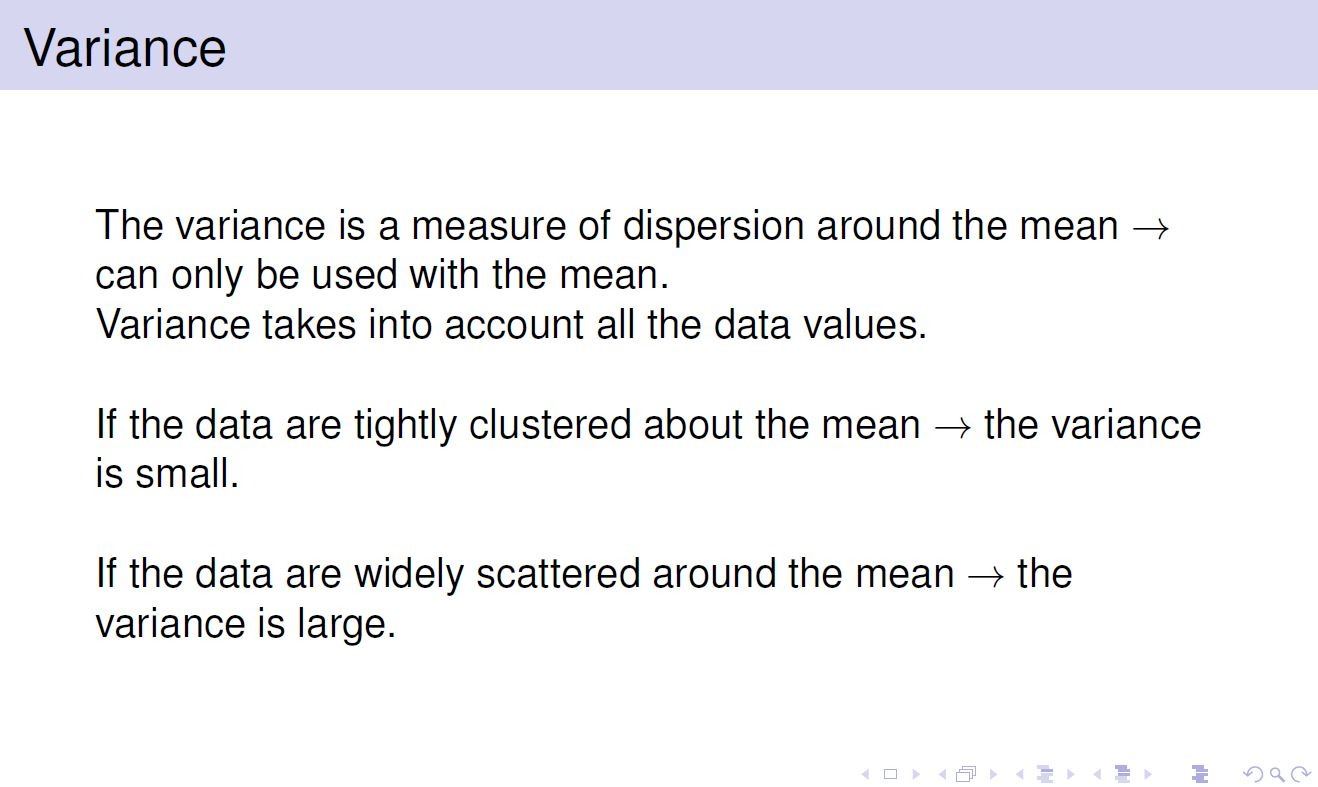
\includegraphics[width=1.1\linewidth]{images/MA4104-Lect04-13}
			
		\end{figure}
	\end{frame}
	%===========================================================%
	\begin{frame}
		\frametitle{Revision of Science Maths 3}
		\begin{figure}
			\centering
			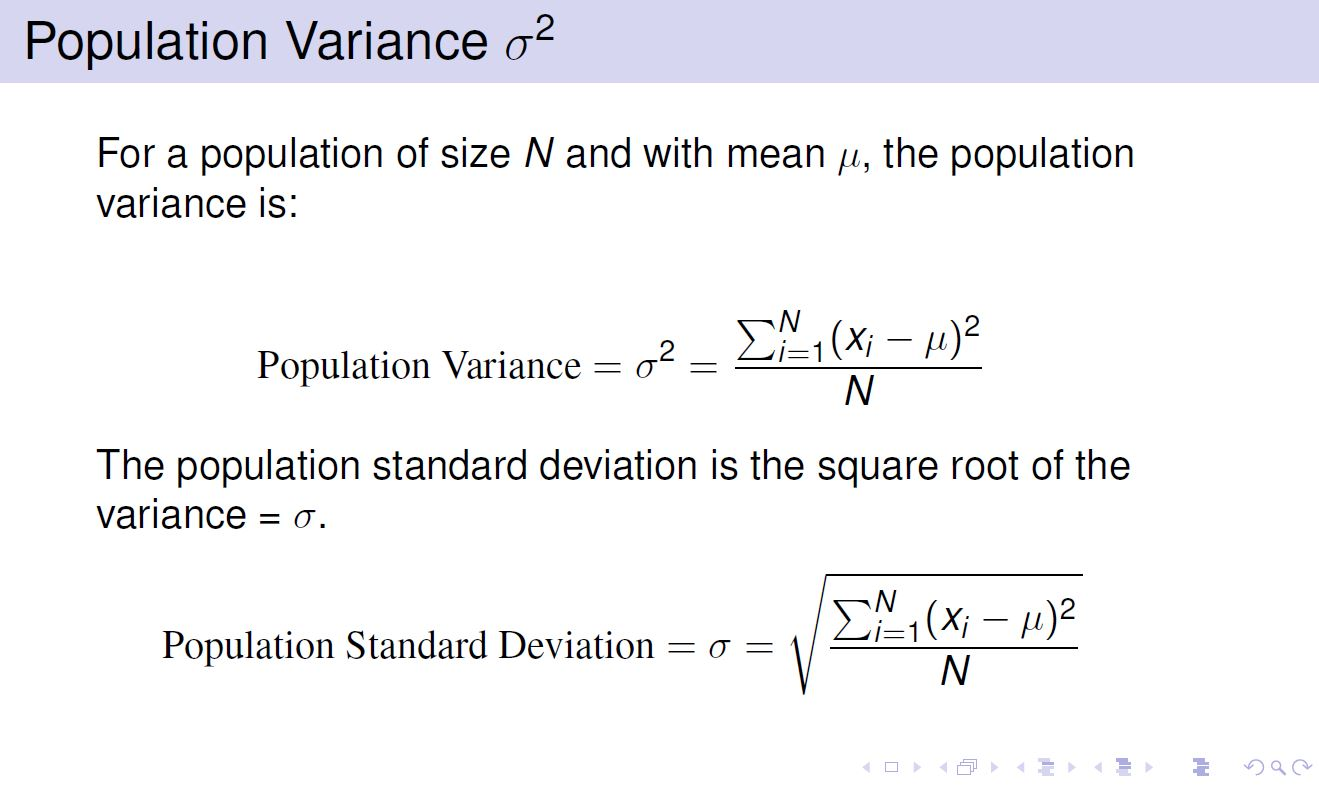
\includegraphics[width=1.1\linewidth]{images/MA4104-Lect04-14}
			
		\end{figure}
	\end{frame}
	%===========================================================%
	\begin{frame}
		\frametitle{Revision of Science Maths 3}
		\begin{figure}
			\centering
			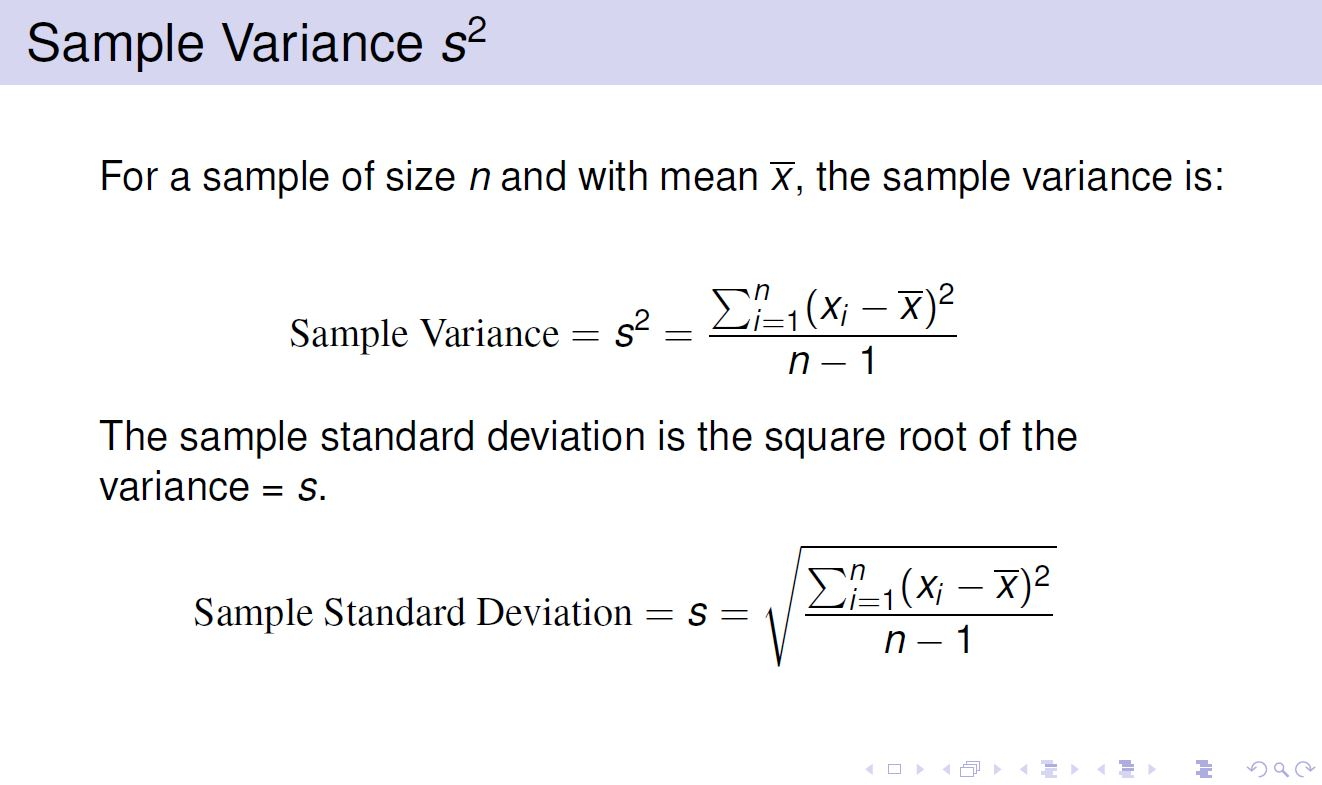
\includegraphics[width=1.1\linewidth]{images/MA4104-Lect04-15}
			
		\end{figure}
	\end{frame}
	%===========================================================%
	\begin{frame}
		\frametitle{Revision of Science Maths 3}
		\begin{figure}
			\centering
			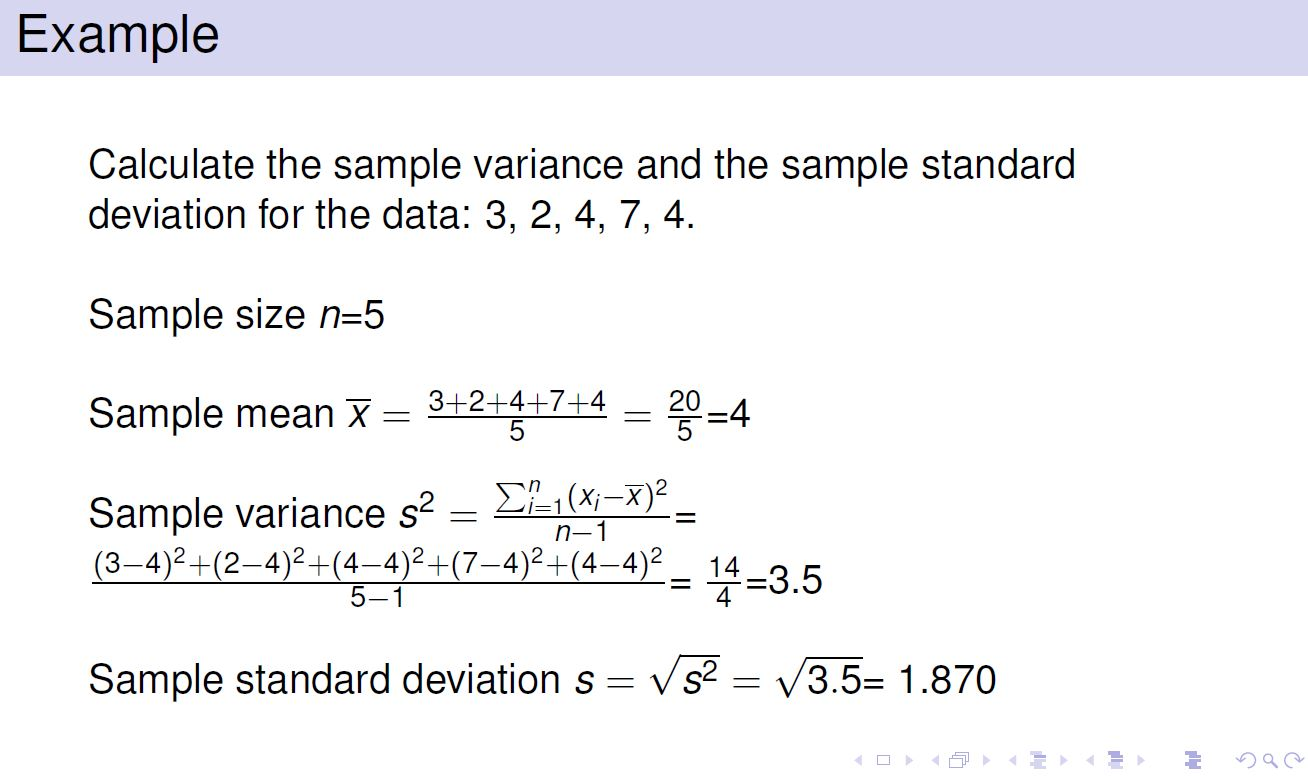
\includegraphics[width=1.1\linewidth]{images/MA4104-Lect04-16}
			
		\end{figure}
	\end{frame}
	%===========================================================%
	\begin{frame}
		\frametitle{Revision of Science Maths 3}
		\begin{figure}
			\centering	
			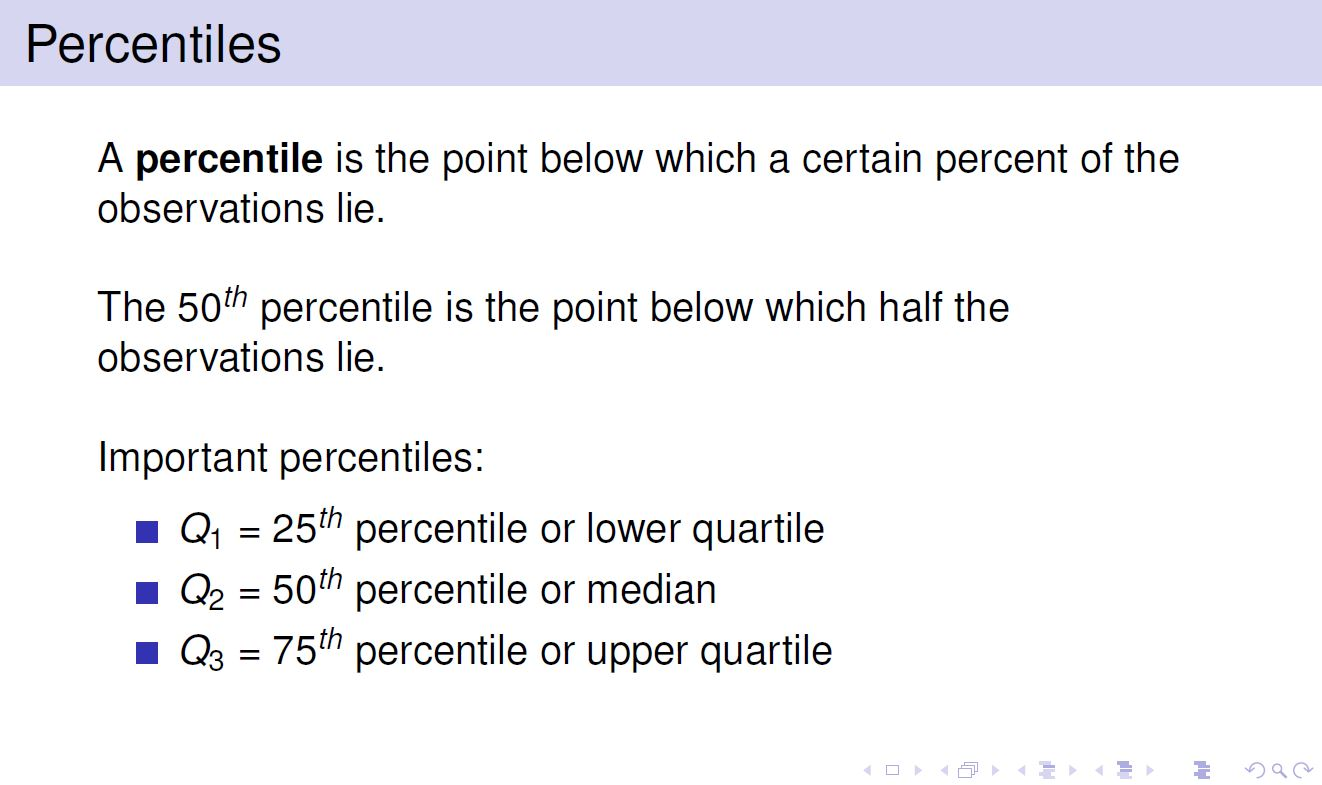
\includegraphics[width=1.1\linewidth]{images/MA4104-Lect04-17}
			
		\end{figure}
	\end{frame}
	%===========================================================%
	\begin{frame}
		\frametitle{Revision of Science Maths 3}
		\begin{figure}
			\centering
			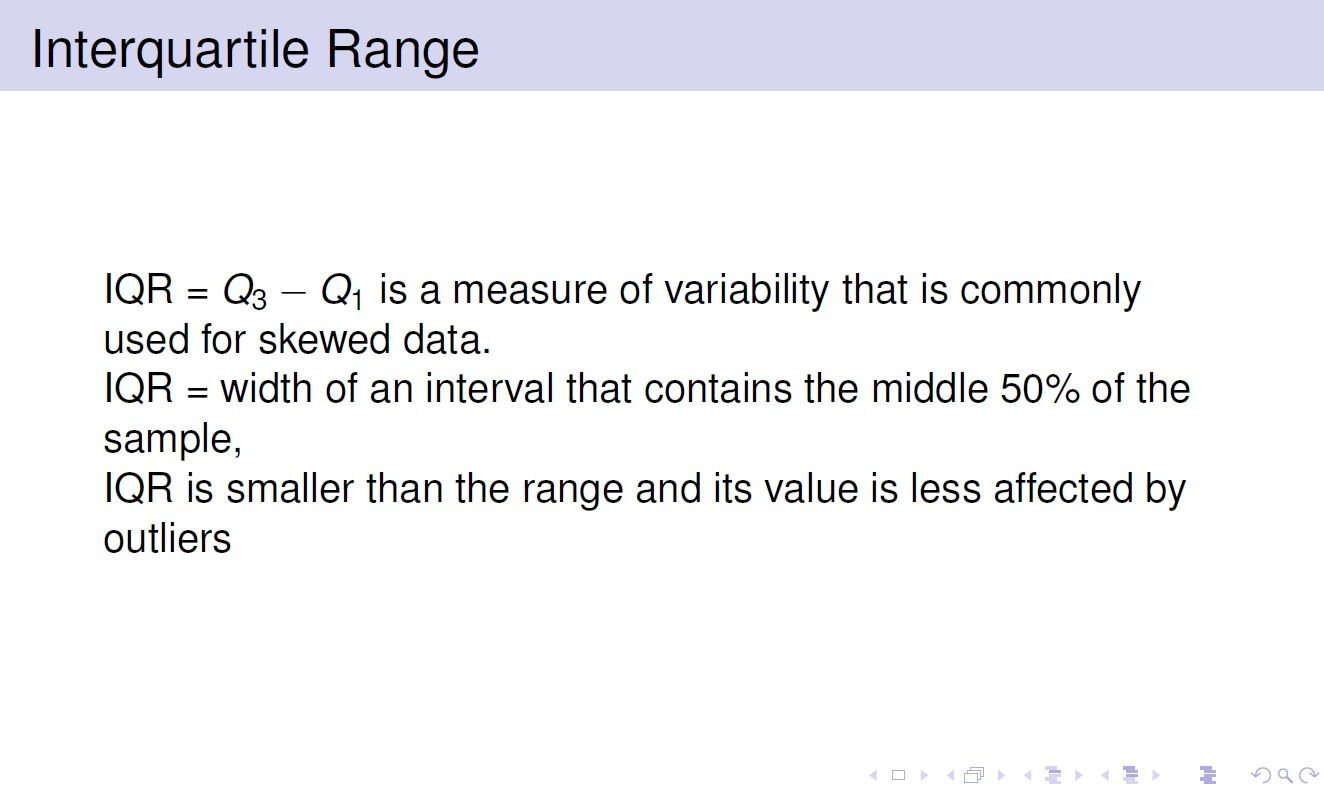
\includegraphics[width=1.1\linewidth]{images/MA4104-Lect04-18}
			
		\end{figure}
	\end{frame}
	
	
		%===========================================================%
		\begin{frame}
			\frametitle{Revision of Science Maths 3}
			\Large
\textbf{Boxplots}
\begin{itemize}
\item	Boxplots are uniform in their use of the box: the bottom and top of the box are always the first and third quartiles, and the band inside the box is the median. 
\item But the ends of the whiskers can represent several possible alternative values (see next slide. We will use the \textbf{Tukey Boxplot} variant). 
\item \textbf{Outliers:} Any data not included between the whiskers should be plotted as an outlier with a dot, small circle, or star, but occasionally this is not done.
\end{itemize}
\end{frame}
		%===========================================================%
		\begin{frame}
			\frametitle{Revision of Science Maths 3}
			\Large
\textbf{Boxplots:} Different ways of computing "Whiskers"
	\begin{itemize}
		\item
	the minimum and maximum of all of the data
\item \textbf{Tukey boxplot}	the lowest datum still within 1.5 IQR of the lower quartile, and the highest datum still within 1.5 IQR of the upper quartile.
\item	one standard deviation above and below the mean of the data
\item	the 9th percentile and the 91st percentile
\item	the 2nd percentile and the 98th percentile.

\end{itemize}
\end{frame}
	
		%===========================================================%
		\begin{frame}
			\frametitle{Revision of Science Maths 3}
\Large
Structure of Boxplot, when no outliers are present
\begin{figure}
\centering
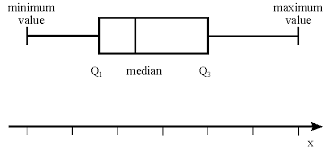
\includegraphics[width=1.0\linewidth]{images/boxplotstructure}
\end{figure}
		\end{frame}
		\begin{frame}
			\frametitle{Revision of Science Maths 3}
\Large
Boxplots can indicate outliers
			\begin{figure}
				\centering
				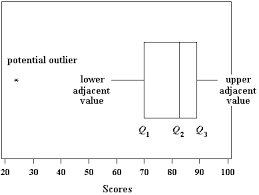
\includegraphics[width=1.0\linewidth]{images/boxplotstructure2}
			\end{figure}
		\end{frame}
				\begin{frame}
					\frametitle{Revision of Science Maths 3}
\begin{figure}
\centering
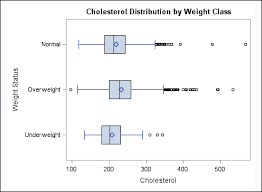
\includegraphics[width=1.0\linewidth]{images/Boxplot}
\end{figure}
				\end{frame}	
	%===========================================================%
	\begin{frame}
		\frametitle{Revision of Science Maths 3}
		\begin{figure}
			\centering
			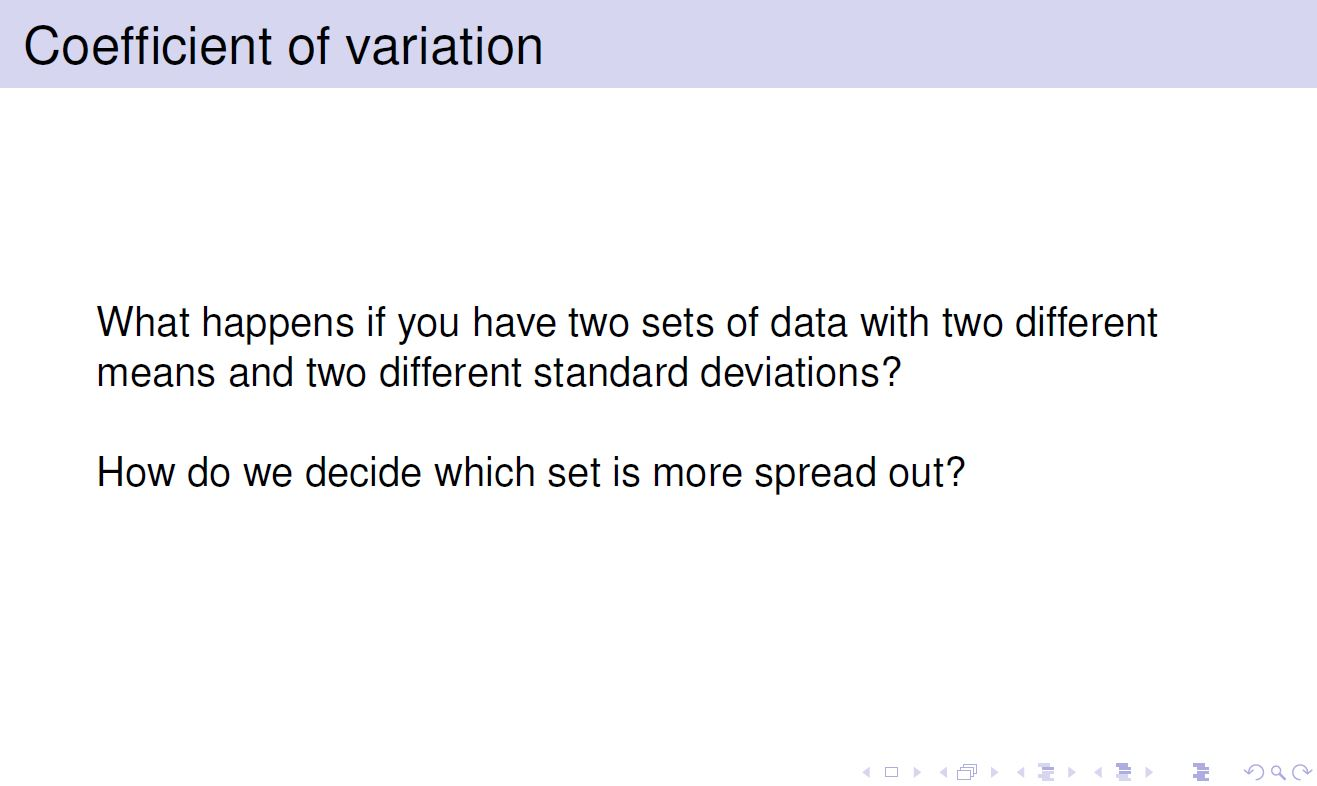
\includegraphics[width=1.1\linewidth]{images/MA4104-Lect04-19}
			
		\end{figure}
	\end{frame}
	%===========================================================%
	\begin{frame}
		\frametitle{Revision of Science Maths 3}
		\begin{figure}
			\centering
			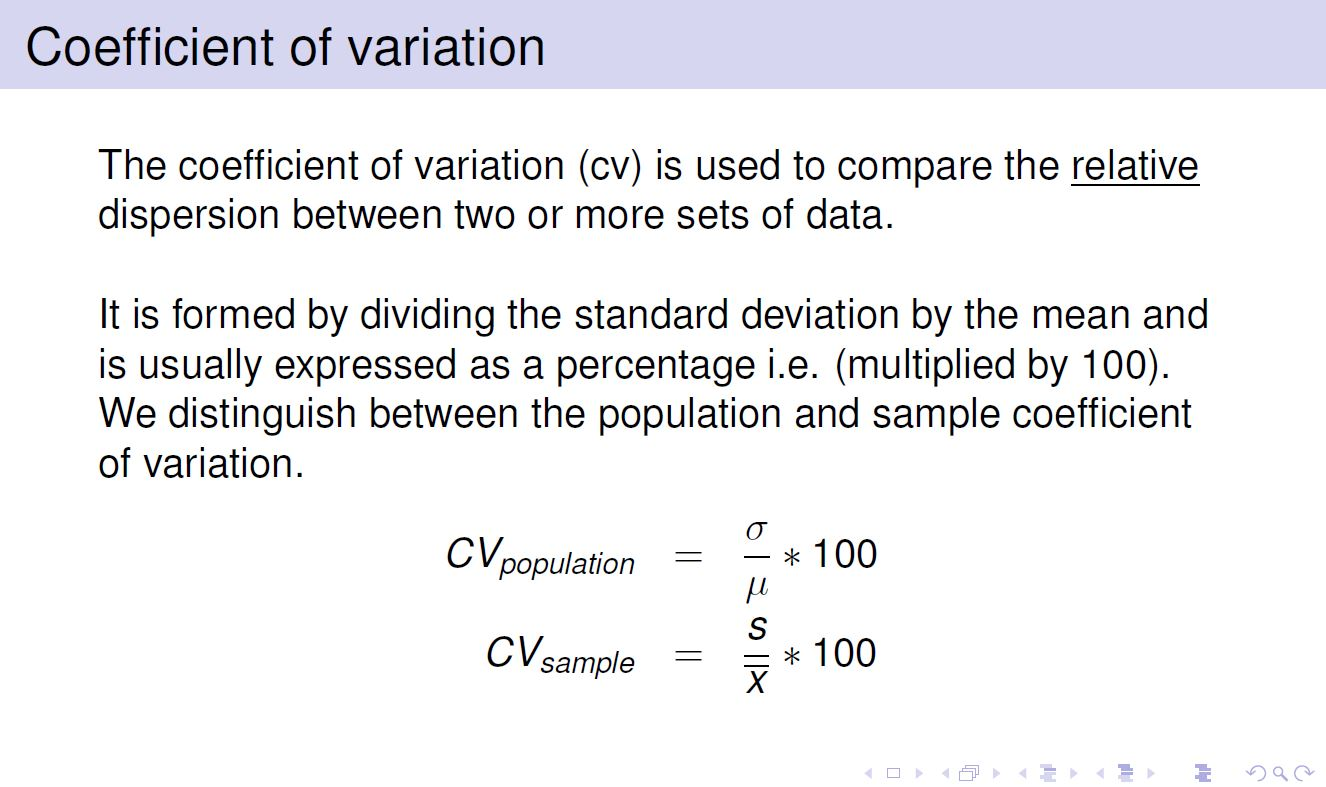
\includegraphics[width=1.1\linewidth]{images/MA4104-Lect04-20}
			
		\end{figure}
	\end{frame}
	
	
	
\end{document}
